\section{What the System Must Do and Its Limits}
\subsection{System functions in plain words}

A small camera watches the driver for four behaviours: yawning, covering the mouth, drinking and using a phone. The system ignores single odd frames and waits until a behaviour is held long enough to be real, then warns the driver with a light and a short voice message stating what it saw, escalating if the behaviour continues. Mirror checks remain silent. Every confirmed event is logged on the device, a display shows the current status and runs the calibration, and after the trip only event records reach a web dashboard of trends and tips, ensuring that no video ever leaves the device. In SDP~2, the system is demonstrated on a desk rig in a room, while the in-car placement remains the target for a vehicle version.

\subsection{List of specifications}
\subsubsection{Functional specifications}

Every Required and Desired feature of Section 1.4 is a numbered, testable specification (FS-01 to FS-26 in Tables \ref{tab:req-features} and \ref{tab:desired-features}), each mapped to a test in Section 5.4. Future features are discussed in Section \ref{sec:future}.

\subsubsection{Performance specifications}

Table \ref{tab:ch4-02} sets a numeric target for the running system, along with how each target is measured.

\begin{table}[htbp]
\centering
\caption{Performance metric targets}
\label{tab:ch4-02}
\footnotesize
\setlength{\tabcolsep}{3pt}
\renewcommand{\arraystretch}{1.15}
\begin{tabular}{|p{0.300\linewidth}|p{0.190\linewidth}|p{0.440\linewidth}|}
\hline
\textbf{Metric} & \textbf{Target} & \textbf{How measured} \\
\hline
Frames per second on the Pi 5 & 25--40+ \gls{fps} & Frame counter averaged over a 30 min live run of the full pipeline after warm-up \\
\hline
End-to-end latency & $\le$ 100 ms & Timestamps at frame capture and at the alert command, reporting the mean and 95th percentile \\
\hline
Per-class recall & 0.90--0.95+ & Confusion matrix on the subject-disjoint test set at the selected cutoffs \\
\hline
False alarms per hour & $\le$ 3 (target), $<$ 10 (minimum) & Confirmed alerts on neutral and hard-negative test clips divided by their duration in hours \\
\hline
Camera-blocked detection & 3 s & Lens covered or dazzled at a random moment, timed to the announcement over 10 trials \\
\hline
Eye-closure alert delay & 1.5 s & Acted eye-closure clips on the demonstration rig, timed from the labelled closure start to the loud alert \\
\hline
\gls{perclos} window & 60 s & Fixed in software and checked with synthetic \gls{ear} sequences \\
\hline
\gls{led} flash rate & $\le$ 3 per second & Toggle timestamps from the log, checked with slow-motion video \\
\hline
Alert cool-down window & 30 s & Two same-class events inside the window, where the second must not alert \\
\hline
Escalation timing & Tier 2 at 5 s, Tier 3 at 10 s & Persistent acted cue, with tier times read from the event log \\
\hline
Human response time to alert & $\le$ 1.5 s & Acted trials on the demonstration rig, from alert start to the visible reaction in video \\
\hline
\end{tabular}
\end{table}

\subsection{List of constraints}

Table \ref{tab:ch4-05} lists the constraints and assumptions that shape the design, along with the specifications each one affects. The system must assist the driver without ever replacing their attention, and a vehicle cabin is harsh on electronics, with power cuts, voltage dips and \gls{uae} heat. Throughout the project, we follow the \gls{ieee} \cite{r66} and \gls{acm} \cite{r67} codes of ethics and the \gls{uae} \gls{pdpl} \cite{r56}.

\begin{table}[htbp]
\centering
\caption{Summary of design constraints}
\label{tab:ch4-05}
\footnotesize
\setlength{\tabcolsep}{3pt}
\renewcommand{\arraystretch}{1.15}
\begin{tabular}{|p{0.170\linewidth}|p{0.290\linewidth}|p{0.300\linewidth}|p{0.160\linewidth}|}
\hline
\textbf{Constraint} & \textbf{Limit / requirement} & \textbf{Effect on the design} & \textbf{Related spec ID} \\
\hline
Economic & 5000 \gls{aed} budget & Required parts first, and the request totals 2725 \gls{aed} & FS-01 to FS-10 \\
\hline
Safety & $\le$ 3 flashes/s, peripheral light, safe volume, clear view & Flash rate capped in software, night dimming, mount away from line of sight & FS-05, FS-14, FS-15 \\
\hline
Security and privacy & No video out, \gls{pin} identity, authenticated \gls{tls} & On-device inference, event-only logs, device key & FS-08, FS-09, FS-19, FS-22 \\
\hline
Reliability & Power cuts, heat, vibration, glare & SQLite \gls{wal}, active cooler, blind check & FS-17, FS-21 \\
\hline
Power and size & 5 V / 5 A, $\le$ 25 W & Power budget with margin, compact vented case & Section \ref{sec:power} \\
\hline
Usability & No interaction while driving, bilingual voice & Short messages, glanceable \gls{ui}, dark mode & FS-16, FS-24 \\
\hline
Ethical and social & Consent, fairness, no surveillance & Authors as subjects, public data for appearance variety, driver owns the data & FS-10, FS-19 \\
\hline
Assumption: setup & Fixed mount, face in view, no sunglasses, enough cabin light, internet only after the trip & \gls{rgb} camera only, SDP~2 testing and demonstration on a desk rig in a room & FS-02, FS-03 \\
\hline
Assumption: scope & Four subjects, four classes, no head-pose model, not certified for vehicles & Visual distraction without an object is not detected & FS-10 \\
\hline
\end{tabular}
\end{table}


\section{Alternative Solutions and How We Chose}

\subsection{Evaluation criteria and why they are ranked this way}

We rank accuracy and false alarms first, since a system that misses events or keeps crying wolf ends up switched off \cite{r28,r10}. Table \ref{tab:ch4-06} gives each weight and how it is measured.

\begin{table}[htbp]
\centering
\caption{Evaluation criteria, weights and how each is measured}
\label{tab:ch4-06}
\footnotesize
\setlength{\tabcolsep}{3pt}
\renewcommand{\arraystretch}{1.15}
\begin{tabular}{|p{0.230\linewidth}|p{0.380\linewidth}|p{0.090\linewidth}|p{0.210\linewidth}|}
\hline
\textbf{Criterion} & \textbf{Why it matters} & \textbf{Weight} & \textbf{How measured} \\
\hline
Accuracy and false alarms & Missed events defeat the purpose, false alarms make drivers switch the system off & 20\% & Recall and false alarms per hour \\
\hline
Real-time speed on the Pi & A late alert is useless, slow frames miss short cues & 18\% & \gls{fps} and latency \\
\hline
Privacy & Video of the driver's face is personal data & 15\% & Whether video leaves the car \\
\hline
Cost & 5000 \gls{aed} budget, low unit cost helps adoption & 14\% & Price in \gls{aed} \\
\hline
Power and heat & Continuous operation in \gls{uae} cabin heat & 12\% & Watts and temperature \\
\hline
Ease of installation & No special tools or wiring skills & 8\% & Parts and steps \\
\hline
Complexity & More parts mean more failure points & 7\% & Build effort estimate \\
\hline
Parts availability & Local purchase keeps the schedule & 6\% & Stock in the \gls{uae} \\
\hline
\end{tabular}
\end{table}

\subsection{Alternative solutions for the whole system}
\subsubsection{Description of each alternative}

Table \ref{tab:ch4-alts} describes the five whole-system alternatives.

\begin{table}[htbp]
\centering
\caption{Whole-system alternatives}
\label{tab:ch4-alts}
\footnotesize
\setlength{\tabcolsep}{3pt}
\renewcommand{\arraystretch}{1.15}
\begin{tabular}{|p{0.050\linewidth}|p{0.230\linewidth}|p{0.320\linewidth}|p{0.330\linewidth}|}
\hline
\textbf{ID} & \textbf{Alternative} & \textbf{How it works} & \textbf{Main weakness} \\
\hline
A & On-device object detection & \gls{yolo}11n on the Pi 5 with the AI HAT+, alerts made in the car & Needs our own dataset, optimisation and cooling \\
\hline
B & Cloud-streamed vision & The car uploads video and a large model runs on a server & Needs a constant connection, adds delay, face video leaves the car \\
\hline
C & Landmark rules & \gls{ear}, mouth opening and head angle with fixed thresholds & Cannot see a phone or a bottle \\
\hline
D & Vehicle signals or wearables & Steering, lane position or heart rate & Indirect, cannot tell what the driver is doing \\
\hline
E & Smartphone app & The phone's camera and processor & Overheats on a sunny dashboard, limited background camera use \\
\hline
\end{tabular}
\end{table}


\subsubsection{Comparison and selected approach}

Figure \ref{fig:ch4-decision} scores each alternative from 1 to 5. Alternative A achieves the highest total (3.96), narrowly ahead of C (3.93). However, C cannot detect phone use, drinking or hand-over-mouth, failing the core requirement FS-03 regardless of its score. The weak points of A are accepted, as each can be handled within SDP~2.

\begin{figure}[htbp]
  \centering
  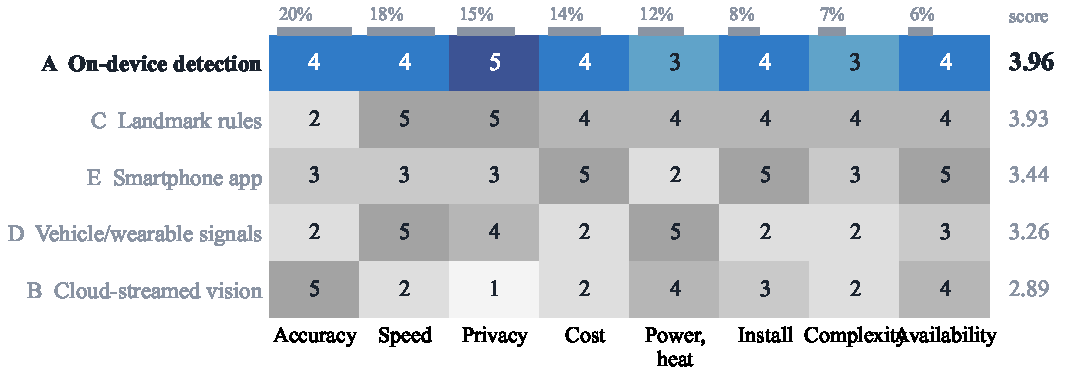
\includegraphics[width=\linewidth]{Figures/heat_decision.pdf}
  \caption{Decision matrix for the whole-system alternatives (scores 1--5, weights above each criterion), sorted by total with the selected design in colour}
  \label{fig:ch4-decision}
\end{figure}

\subsection{Alternatives for each major part}
\subsubsection{Processing platform}

On the Pi 5 CPU alone, \gls{yolo}11n reaches only 6.79 \gls{fps} \cite{r52}, so we add the AI HAT+ to move detection onto an \gls{npu}. Table \ref{tab:ch4-08} compares the options.

\begin{table}[htbp]
\centering
\caption{Processing platform options}
\label{tab:ch4-08}
\footnotesize
\setlength{\tabcolsep}{3pt}
\renewcommand{\arraystretch}{1.15}
\begin{tabular}{|p{0.200\linewidth}|p{0.120\linewidth}|p{0.100\linewidth}|p{0.170\linewidth}|p{0.150\linewidth}|p{0.180\linewidth}|}
\hline
\textbf{Option} & \textbf{Price (\gls{aed})} & \textbf{Power (W)} & \textbf{Expected \gls{fps}} & \textbf{\gls{uae} availability} & \textbf{Verdict} \\
\hline
Raspberry Pi 5 (CPU only) & 845 & 5--12 & 6.8 at 640 \cite{r52} & Good & Fallback only \\
\hline
Pi 5 with AI HAT+ & 845 + 391 & +2--3 & $\ge$ 30 (to be measured) & Good & \textbf{Selected} \\
\hline
Jetson Orin Nano & About 900--1100 & 7--25 & $\ge$ 30 & Limited & Too costly, more heat \\
\hline
Raspberry Pi 4 & About 300 & 4--7 & Below 5 & Good & Too slow \\
\hline
\end{tabular}
\end{table}

\subsubsection{Camera}

A \gls{usb} \gls{rgb} webcam is plug-and-play and matches the public \gls{rgb} data we pre-train on. An \gls{ir} camera performs better at night and remains a Future item (Table \ref{tab:ch4-09}).

\begin{table}[htbp]
\centering
\caption{Camera options}
\label{tab:ch4-09}
\footnotesize
\setlength{\tabcolsep}{3pt}
\renewcommand{\arraystretch}{1.15}
\begin{tabular}{|p{0.200\linewidth}|p{0.180\linewidth}|p{0.200\linewidth}|p{0.120\linewidth}|p{0.210\linewidth}|}
\hline
\textbf{Option} & \textbf{Resolution / \gls{fps}} & \textbf{Night performance} & \textbf{Cost (\gls{aed})} & \textbf{Verdict} \\
\hline
\gls{usb} \gls{uvc} \gls{rgb} (C922) & 1080p at 30 & Poor without cabin light & 255 & \textbf{Selected} \\
\hline
\gls{ir} / \gls{nir} camera & 720p--1080p at 30 & Good with illuminators & 150--400 & Future \\
\hline
Pi camera (CSI) & Up to 12 MP & Good with NoIR variant & About 120--150 & Short ribbon, awkward to mount \\
\hline
Dashcam & 1080p+ & Varies & 200+ & Closed firmware, no live stream \\
\hline
\end{tabular}
\end{table}

\subsubsection{Detection model}

\gls{yolo}11n offers the best balance of size and accuracy among models with a mature path to the Hailo \gls{npu}, with \gls{yolo}26n kept as a backup should its \gls{npu} export mature (Table \ref{tab:ch4-10}).


\begin{table}[htbp]
\centering
\caption{Detection model candidates (\glsentryshort{coco}, 640 px)}
\label{tab:ch4-10}
\footnotesize
\setlength{\tabcolsep}{3pt}
\renewcommand{\arraystretch}{1.15}
\begin{tabular}{|p{0.170\linewidth}|p{0.120\linewidth}|p{0.120\linewidth}|p{0.170\linewidth}|p{0.170\linewidth}|p{0.150\linewidth}|}
\hline
\textbf{Model} & \textbf{Params (M)} & \textbf{GFLOPs} & \textbf{\gls{map}$_{50-95}$} & \textbf{Pi 5 CPU \gls{fps}} & \textbf{Licence} \\
\hline
\textbf{\gls{yolo}11n} \cite{r45} & 2.6 & 6.5 & 39.5 & 6.8 \cite{r52} & AGPL-3.0 \\
\hline
\gls{yolo}v8n & 3.2 & 8.7 & 37.3 & SDP~2 & AGPL-3.0 \\
\hline
\gls{yolo}11s & 9.4 & 21.6 & 47.0 & SDP~2 & AGPL-3.0 \\
\hline
\gls{yolo}v10n \cite{r71} & 2.3 & 6.7 & 38.5 & SDP~2 & AGPL-3.0 \\
\hline
\gls{yolo}26n \cite{r76} & 2.4 & 5.5 & 40.9 & 7.8 \cite{r52} & AGPL-3.0 \\
\hline
\end{tabular}
\end{table}

\subsubsection{Remaining components}

Table \ref{tab:ch4-parts} lists the remaining parts. A light bar paired with a voice message is preferred over a buzzer, which cannot explain itself, and over a screen, which pulls the eyes off the road \cite{r20,r22}. The PXN wheel serves as the steering wheel of the desk demonstration rig and prototypes a Future vibration alert.

\begin{table}[htbp]
\centering
\caption{Remaining components, alternatives and electrical specifications}
\label{tab:ch4-parts}
\footnotesize
\setlength{\tabcolsep}{3pt}
\renewcommand{\arraystretch}{1.15}
\begin{tabular}{|p{0.120\linewidth}|p{0.170\linewidth}|p{0.190\linewidth}|p{0.250\linewidth}|p{0.200\linewidth}|}
\hline
\textbf{Part} & \textbf{Selected (\gls{aed})} & \textbf{Alternatives} & \textbf{Why selected} & \textbf{Key electrical spec} \\
\hline
Audio alert & Creative Pebble V3 (177) & Buzzer, 3.5 mm speaker with amplifier & Clear voice messages, no amplifier board, \gls{usb} powered & 5 V \gls{usb}, \gls{usb} audio class \\
\hline
Visual alert & \gls{rgb} light bar (70) & Single \gls{led}, strobe beacon & Visible in peripheral vision, one colour per class & 5 V, about 0.3 A, switched by \gls{mosfet} \\
\hline
Driver display & Hosyond 7-inch touch (245) & Phone over Wi-Fi, 20$\times$4 character \gls{lcd} & Room for status and calibration screens, no extra radio & 5 V, about 0.5 A, \gls{hdmi} and \gls{usb} touch \\
\hline
Power supply & Official 27 W PD (112) & 5 V / 3 A supply, power bank & Only a 5 A supply raises the \gls{usb} limit to 1.6 A & 5.1 V, 5 A, \gls{usb}-C PD \\
\hline
Storage & SanDisk Extreme Pro 128 GB (136) & \gls{usb} SSD, basic microSD & Fast and durable, low write load from events only & A2, U3 microSD \\
\hline
Cooling and case & Active Cooler (64), metal case (86) & Passive heatsink, plastic case & Keeps the Pi below throttling under \gls{npu} load & Fan powered and controlled by the Pi \\
\hline
\gls{usb} hub & UGREEN 3.0 hub (28) & Pi ports only & Four \gls{usb} devices on the Pi's ports & Bus powered, shares the 1.6 A \\
\hline
Light switch & Logic-level \gls{mosfet} (lab stock) & Relay module, BJT & Silent, fast \gls{pwm}, fully on at 3.3 V gate drive & Gate threshold 1--2 V \\
\hline
Server and maps & FastAPI, PostgreSQL and React on a free tier & Paid map \gls{api}, managed backend & Free and open source, and Overpass needs no key \cite{r68} & HTTPS with \gls{tls} 1.3 \\
\hline
\end{tabular}
\end{table}


\section{The Selected Design: Technical Approach}

\subsection{System overview: the big picture}
\subsubsection{Overall block diagram}

Figure \ref{fig:ch4-03} presents the whole system. Before deployment, the model is trained, hardened with hard negatives and compiled for the \gls{npu}. During a session, frames flow from the camera through the detector and the \gls{ema} into the decision block, the only place where scores turn into alerts. After the session, only event records leave the device. The driver display acts as both an output and an input, since calibration writes the cutoffs that the decision block uses.


\begin{sidewaysfigure}
\centering
\resizebox{\textheight}{!}{%
\begin{tikzpicture}[font=\footnotesize, >={Triangle[length=2.6mm,width=2.6mm]}, arr/.style={->, line width=1.3pt},
  lab/.style={font=\scriptsize\bfseries, fill=white, inner sep=1.5pt}]
  % ---------------- pre-deployment (top)
  \sysblock{p1}{sbgray}{\faVideo}{Dataset collection}{Subject-disjoint in-cabin \gls{rgb} clips, four cues}{at={(0,6.4)}}
  \sysblock{p2}{sbgray}{\faTimesCircle}{Hard negatives}{Look-alikes of the same subjects, negatives only}{at={(4.6,6.4)}}
  \sysblock{p3}{sbgray}{\faCubes}{Train and compile}{Fine-tune, prune, \gls{int} quantise for the \gls{npu}}{at={(9.2,6.4)}}
  \foreach \n/\k in {p1/1,p2/2,p3/3} \sysnum{\n}{sbgray}{\k}
  \draw[arr] (p1) -- (p2); \draw[arr] (p2) -- (p3);
  \begin{scope}[on background layer]
    \node[draw=gray, dotted, line width=1.1pt, fill=gray!10, inner sep=6mm, fit=(p1)(p3), label={[anchor=south west, font=\small]north west:Pre-deployment}] (pre) {};
  \end{scope}
  % ---------------- real time (middle)
  \sysblock{r1}{sbblue}{\faCamera}{Camera feed}{C922, 1080p at 30 \gls{fps}}{at={(0,0)}}
  \sysblock{r2}{sbblue}{\faCrop}{Crop and blind check}{400$\times$400 RoI crop, brightness, sharpness}{at={(4.6,0)}}
  \sysblock{r3}{sbblue}{\faProjectDiagram}{\gls{yolo}11n on AI HAT+}{Box and score per class}{at={(9.2,0)}}
  \sysblock{r4}{sbblue}{\faFilter}{\gls{ema} filter}{Per-class $\tau$ in seconds}{at={(13.8,0)}}
  \sysblock{r5}{sbblue}{\faBalanceScale}{Decision}{Cutoff, confirm time, cool-down, tier}{at={(18.4,0)}}
  \sysblock{r6}{sbred}{\faBell}{Alert}{Light bar, chime or voice, explained message}{at={(23.4,1.5)}}
  \sysblock{r7}{sbblue}{\faDatabase}{Event log}{SQLite \gls{wal}, events only}{at={(23.4,-1.6)}}
  \sysblock{r8}{sbblue}{\faTablet}{Driver display}{Status, \gls{pin}, calibration}{at={(13.8,-3.3)}, dashed}
  \foreach \n/\k in {r1/1,r2/2,r3/3,r4/4,r5/5,r7/7,r8/8} \sysnum{\n}{sbblue}{\k}
  \sysnum{r6}{sbred}{6}
  \draw[arr] (r1) -- (r2); \draw[arr] (r2) -- (r3); \draw[arr] (r3) -- (r4); \draw[arr] (r4) -- (r5);
  \draw[arr] (r5.east) -- ++(5mm,0) |- (r6.west); \draw[arr] (r5.east) -- ++(5mm,0) |- (r7.west);
  \draw[arr, dashed] (r8.east) -| node[pos=0.25, lab]{cutoffs} (r5.south);
  \draw[arr] (p3.south) -- node[pos=0.55, lab]{Compiled model (.hef)} (r3.north);
  \begin{scope}[on background layer]
    \node[draw=sbblue, dotted, line width=1.1pt, fill=blue!4, inner sep=6mm, fit=(r1)(r6)(r7)(r8), label={[anchor=south west, font=\small]north west:In the vehicle, during the drive}] (rt) {};
  \end{scope}
  % ---------------- server (bottom)
  \sysblock{s1}{sbgreen}{\faCloud}{Upload}{After the trip, \gls{tls}, events only}{at={(23.4,-8.2)}}
  \sysblock{s2}{sbgreen}{\faServer}{Server database}{Deduplicated by event ID}{at={(18.4,-8.2)}}
  \sysblock{s3}{sbgreen}{\faChartLine}{Web dashboard}{Trends, heatmap, post-trip tips}{at={(13.8,-8.2)}}
  \foreach \n/\k in {s1/9,s2/10,s3/11} \sysnum{\n}{sbgreen}{\k}
  \draw[arr] (s1) -- (s2); \draw[arr] (s2) -- (s3);
  \draw[arr, sbblue] (r7.south) -- node[lab, pos=0.5]{Only event records leave the vehicle} (s1.north);
  \begin{scope}[on background layer]
    \node[draw=sbgreen, dotted, line width=1.1pt, fill=green!5, inner sep=6mm, fit=(s1)(s3), label={[anchor=south west, font=\small]north west:On the server, after the session}] (srv) {};
  \end{scope}
  % ---------------- driver (left)
  \sysblock{d1}{sbgold}{\faUser}{Driver}{Monitored, hears explained alerts, reviews the dashboard}{at={(-6.2,0)}}
  \begin{scope}[on background layer]
    \node[draw=sbgold, dashed, line width=1.1pt, fill=yellow!6, inner sep=4mm, fit=(d1)] (drv) {};
  \end{scope}
  \draw[arr, sbred] (r6.north) -- (r6.north |- 0,4.2) -- node[pos=0.5, lab]{Alerts the driver} (drv.north |- 0,4.2) -- (drv.north);
  \draw[arr] (drv.east) -- (r1.west);
  \draw[arr, sbgreen] (s3.west) -- node[pos=0.5, lab]{Improves behaviour} (drv.south |- s3.west) -- (drv.south);
  % legend
  \node[draw, line width=0.8pt, minimum width=8mm, minimum height=4mm] (lg1) at (-7.4,-7.6) {};
  \node[right=1mm of lg1, font=\scriptsize] {Required};
  \node[draw, dashed, line width=0.8pt, minimum width=8mm, minimum height=4mm, below=3mm of lg1] (lg2) {};
  \node[right=1mm of lg2, font=\scriptsize] {Desired};
\end{tikzpicture}}
\caption{System block diagram, where only event records cross from the vehicle to the server}
\label{fig:ch4-03}
\end{sidewaysfigure}

\subsection{How the system operates step by step}

At power-on, the Pi checks its devices, the driver enters a \gls{pin}, and a new driver completes the 20\,s calibration of Section \ref{sec:calib} (Figure \ref{fig:ch4-11}). Each frame is then checked, cropped, scored and smoothed, and a cue is confirmed only once it stays above the cutoff for its confirmation time (Figure \ref{fig:ch4-12}). The system fails safe: a blocked view is announced, missing eyes are skipped rather than counted as open, and a power cut never corrupts the log. After the session, unsent events are uploaded over \gls{tls} whenever Wi-Fi is available.

\begin{figure}[htbp]
  \centering
  \resizebox{!}{0.78\textheight}{\begin{tikzpicture}[node distance=6mm and 10mm]
  % start-up
  \fterm{a}{sbgray}{Power on}{}
  \fcard{b}{sbgray}{\faPowerOff}{Boot and self-check: camera, speaker, light bar}{below=of a}
  \fdec{c}{sbgray}{Self-check ok?}{below=of b}
  \fcard{c1}{sbred}{\faVolumeUp}{Voice: device fault, log and retry}{left=of c}
  \fcard{d}{sbblue}{\faKeyboard}{Driver enters PIN}{below=of c, dashed}
  \fdec{e}{sbblue}{Known driver?}{below=of d}
  \fcard{f}{sbblue}{\faUserCheck}{20\,s calibration}{right=of e, dashed}
  \fcard{g}{sbblue}{\faSlidersH}{Load the driver's cutoffs}{below=of e}
  % drive
  \fcard{h}{sbblue}{\faSync}{Detection and alert loop (Figure \ref{fig:ch4-12})}{below=20mm of g}
  \fdec{i}{sbblue}{Session ended?}{below=of h}
  % after the drive
  \fcard{j}{sbgreen}{\faSave}{Flush and checkpoint the log}{below=20mm of i}
  \fdec{k}{sbgreen}{Wi-Fi available?}{below=of j}
  \fcard{l}{sbgreen}{\faCloud}{\gls{tls} upload of events}{right=of k, dashed}
  \fterm{m}{sbgreen}{Shutdown}{below=of k}

  \draw[farr] (a) -- (b); \draw[farr] (b) -- (c);
  \draw[farr] (c) -- node[flab, right]{yes} (d);
  \draw[farr] (c) -- node[flab, above]{no} (c1);
  \draw[farr] (c1.north) |- (b.west);
  \draw[farr] (d) -- (e);
  \draw[farr] (e) -- node[flab, right]{yes} (g);
  \draw[farr] (e) -- node[flab, above]{no} (f);
  \draw[farr] (f.south) |- (g.east);
  \draw[farr] (g) -- (h); \draw[farr] (h) -- (i);
  \draw[farr] (i) -- node[flab, left, pos=0.3]{yes} (j);
  \draw[farr] (i.west) -- node[flab, above]{no} ++(-14mm,0) |- (h.west);
  \draw[farr] (j) -- (k);
  \draw[farr] (k) -- node[flab, above]{yes} (l);
  \draw[farr] (k) -- node[flab, right]{no} (m);
  \draw[farr] (l.south) |- (m.east);

  \coordinate (iw) at ([xshift=-14mm]i.west);
  \begin{scope}[on background layer]
    \node[freg=sbgray, fit=(a)(c1)(f)(g), label={[freglab]north west:Start-up}] {};
    \node[freg=sbblue, fit=(h)(i)(iw), label={[freglab]north west:During the drive}] {};
    \node[freg=sbgreen, fit=(j)(l)(m), label={[freglab]north west:After the drive}] {};
  \end{scope}
\end{tikzpicture}
}
  \caption{Top-level system flowchart (dashed: Desired)}
  \label{fig:ch4-11}
\end{figure}

\begin{figure}[htbp]
  \centering
  \resizebox{\linewidth}{!}{\begin{tikzpicture}[node distance=6mm and 10mm]
  % every frame
  \fcard{g}{sbblue}{\faCamera}{Grab 1080p frame, measure $\Delta t$}{}
  \fdec{b}{sbblue}{Blocked for 3\,s?}{below=of g}
  \fcard{bb}{sbred}{\faVolumeUp}{Voice: camera blocked, pause, log}{left=of b}
  \fcard{c}{sbblue}{\faCrop}{640$\times$640 crop}{below=of b}
  \fcard{y}{sbblue}{\faProjectDiagram}{\gls{yolo}11n on the \gls{npu}}{below=of c}
  \fcard{e}{sbblue}{\faFilter}{Max score per class, \gls{ema} update}{below=of y}
  % decision
  \fdec{d1}{sbred}{Above cutoff?}{right=26mm of g}
  \fdec{d2}{sbred}{Held for confirm time?}{below=of d1}
  \fdec{d3}{sbred}{In cool-down?}{below=of d2}
  \fcard{t}{sbred}{\faLayerGroup}{Select tier from duration and recent events}{below=of d3}
  \fcard{a}{sbred}{\faBell}{Light pattern and explained voice message}{below=of t}
  \fcard{l}{sbblue}{\faDatabase}{Write event to SQLite}{below=of a}

  \coordinate (top) at ($(g.north)+(0,14mm)$);
  \coordinate (lane) at ($(d1.east)+(9mm,0)$);
  \draw[farr] (g) -- (b);
  \draw[farr] (b) -- node[flab, right]{no} (c);
  \draw[farr] (b) -- node[flab, above]{yes} (bb);
  \draw[farr] (bb.north) |- (g.west);
  \draw[farr] (c) -- (y); \draw[farr] (y) -- (e);
  \draw[farr] (e.east) -- ++(8mm,0) |- (d1.west);
  \draw[farr] (d1) -- node[flab, right]{yes} (d2);
  \draw[farr] (d2) -- node[flab, right]{yes} (d3);
  \draw[farr] (d3) -- node[flab, right]{no} (t);
  \draw[farr] (t) -- (a); \draw[farr] (a) -- (l);
  % return lane to the next frame
  \draw[fline] (d1.east) -- node[flab, above]{no} (d1.east -| lane);
  \draw[fline] (d2.east) -- node[flab, above]{no} (d2.east -| lane);
  \draw[fline] (d3.east) -- node[flab, above]{yes} (d3.east -| lane);
  \draw[fline] (l.east) -- (l.east -| lane);
  \draw[farr] (l.east -| lane) -- (lane |- top) -- node[flab, above, pos=0.5]{next frame} (top) -- (g.north);

  % letters tie the steps to the worked example below
  \linknum{e.north west}{}{A}
  \linknum{d1.west}{}{B}
  \linknum{d2.west}{}{C}
  \linknum{a.north west}{}{D}

  % worked example: one yawn, frame by frame
  \begin{scope}[shift={($(bb.west |- l.south)+(30mm,-37mm)$)}, font=\small]
    \node[inner sep=0, anchor=south west] at (0.030,0.950) {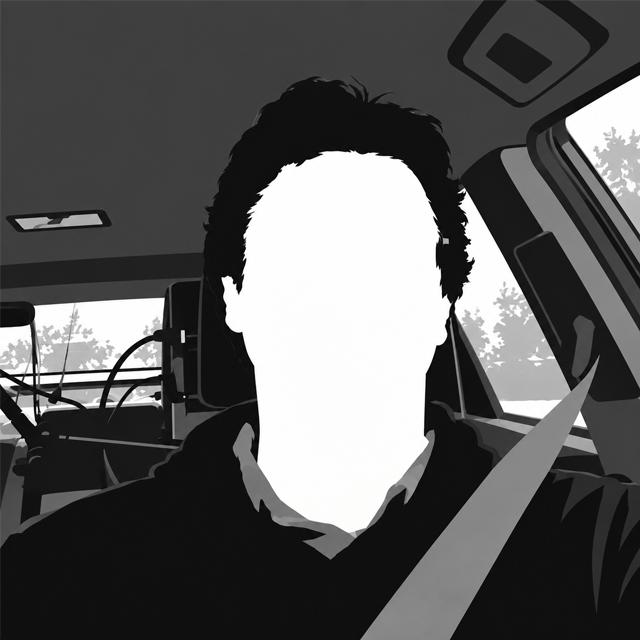
\includegraphics[width=1.940cm,height=1.940cm]{Figures/guide_0.png}};
\node[inner sep=0, anchor=south west] at (2.030,0.950) {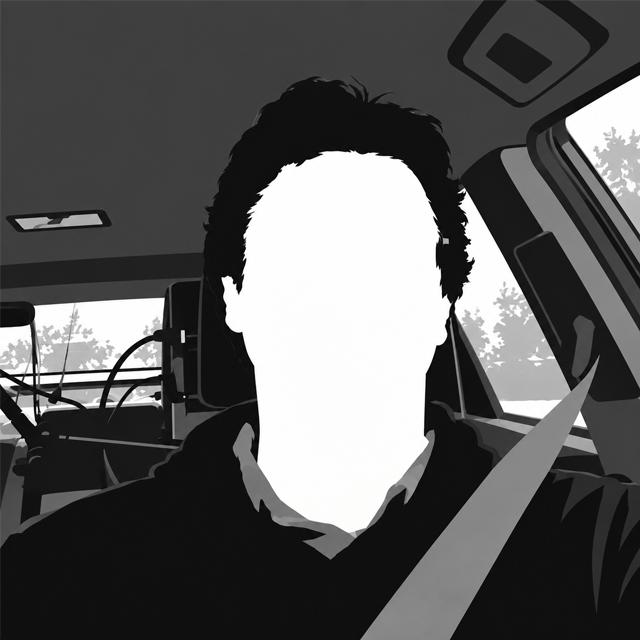
\includegraphics[width=1.940cm,height=1.940cm]{Figures/guide_0.png}};
\node[inner sep=0, anchor=south west] at (4.030,0.950) {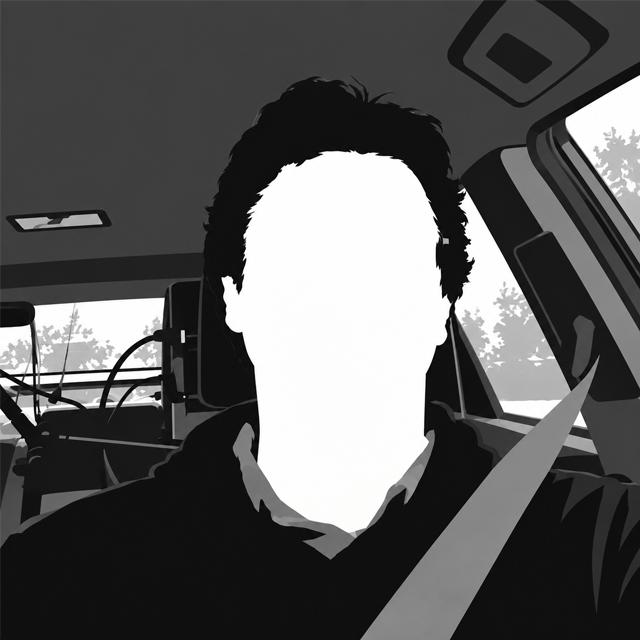
\includegraphics[width=1.940cm,height=1.940cm]{Figures/guide_0.png}};
\node[inner sep=0, anchor=south west] at (6.030,0.950) {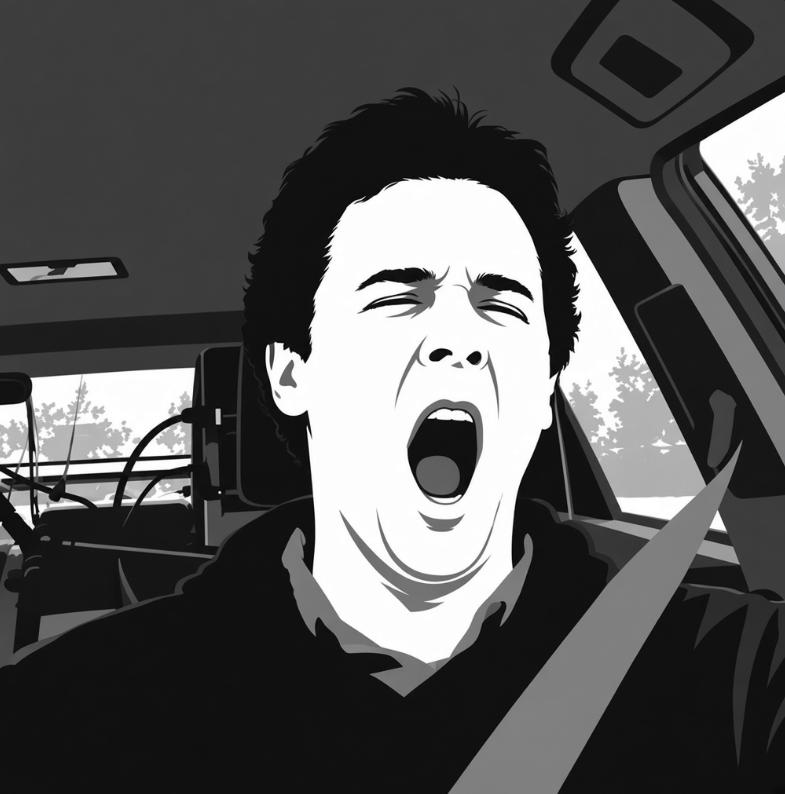
\includegraphics[width=1.940cm,height=1.940cm]{Figures/guide_2.png}};
\node[inner sep=0, anchor=south west] at (8.030,0.950) {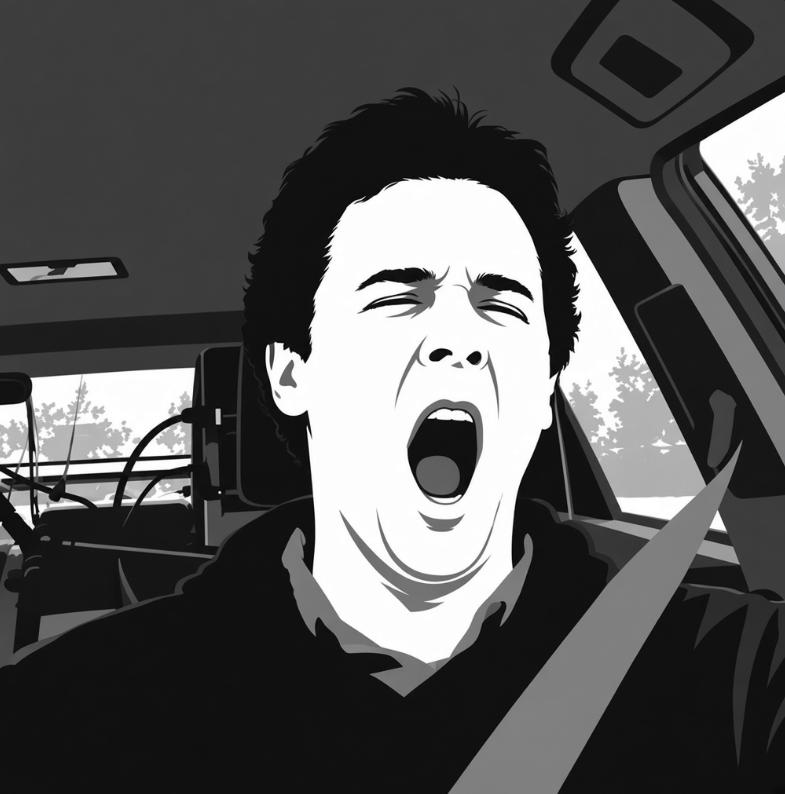
\includegraphics[width=1.940cm,height=1.940cm]{Figures/guide_2.png}};
\node[inner sep=0, anchor=south west] at (10.030,0.950) {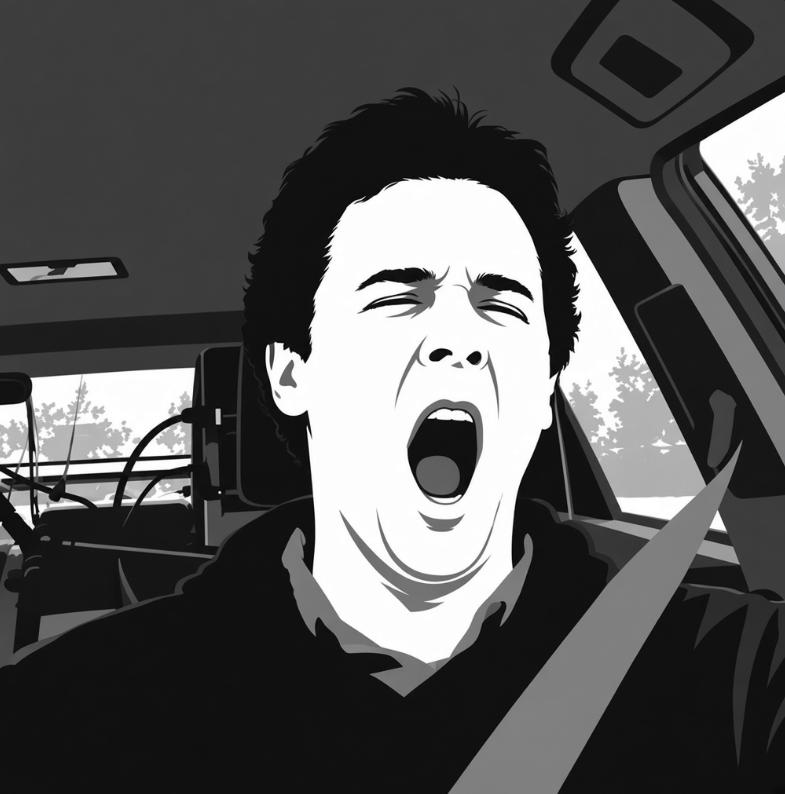
\includegraphics[width=1.940cm,height=1.940cm]{Figures/guide_2.png}};
\node[inner sep=0, anchor=south west] at (12.030,0.950) {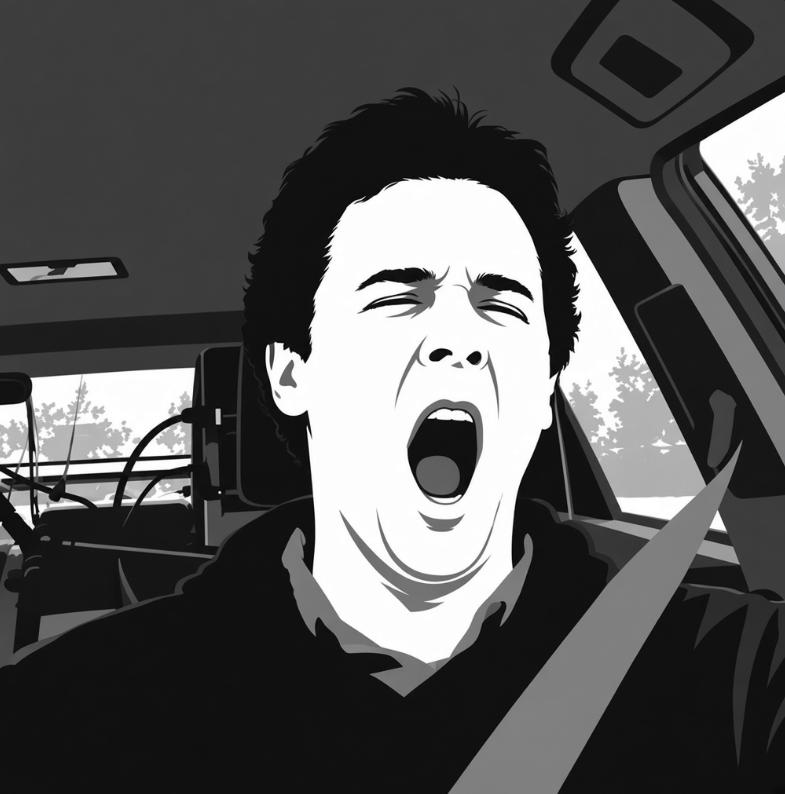
\includegraphics[width=1.940cm,height=1.940cm]{Figures/guide_2.png}};
\node[inner sep=0, anchor=south west] at (14.030,0.950) {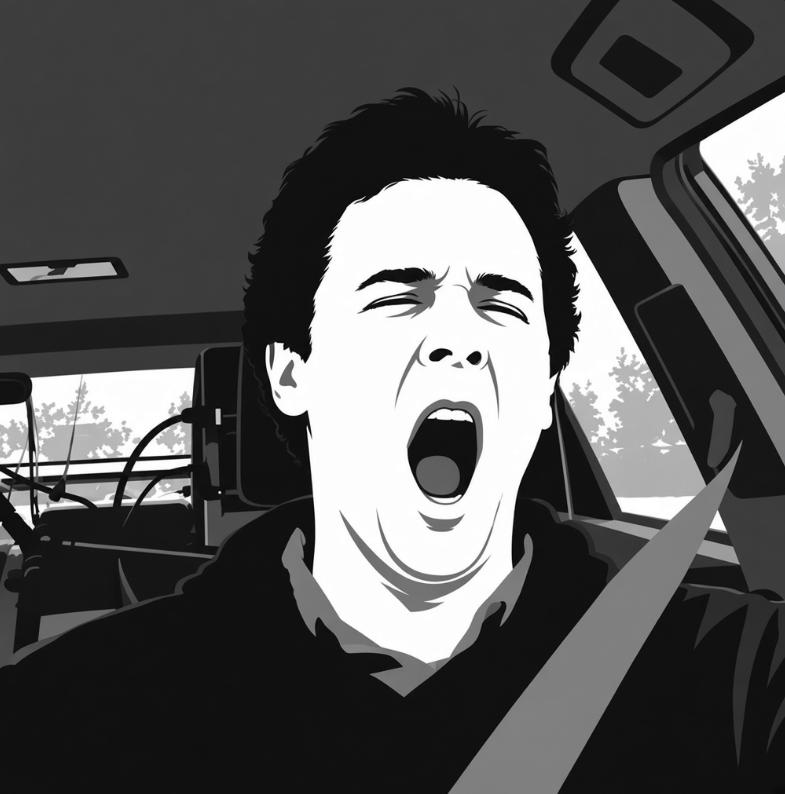
\includegraphics[width=1.940cm,height=1.940cm]{Figures/guide_2.png}};
\node[anchor=east] at (-0.15,1.950) {Frames};
\node[anchor=east] at (-0.15,0.210) {Raw score $x_t$};
\node[anchor=east] at (-0.15,-0.510) {Smoothed $s_t$};
\node[anchor=east] at (-0.15,-1.230) {$s_t > \theta$};
\filldraw[draw=white, line width=0.6pt, fill=sbblue!6!white] (0.000,0.000) rectangle ++(0.400,0.420);
\filldraw[draw=white, line width=0.6pt, fill=sbblue!1!white] (0.000,-0.720) rectangle ++(0.400,0.420);
\filldraw[draw=white, line width=0.6pt, fill=gray!12] (0.000,-1.440) rectangle ++(0.400,0.420);
\filldraw[draw=white, line width=0.6pt, fill=sbblue!7!white] (0.400,0.000) rectangle ++(0.400,0.420);
\filldraw[draw=white, line width=0.6pt, fill=sbblue!2!white] (0.400,-0.720) rectangle ++(0.400,0.420);
\filldraw[draw=white, line width=0.6pt, fill=gray!12] (0.400,-1.440) rectangle ++(0.400,0.420);
\filldraw[draw=white, line width=0.6pt, fill=sbblue!5!white] (0.800,0.000) rectangle ++(0.400,0.420);
\filldraw[draw=white, line width=0.6pt, fill=sbblue!2!white] (0.800,-0.720) rectangle ++(0.400,0.420);
\filldraw[draw=white, line width=0.6pt, fill=gray!12] (0.800,-1.440) rectangle ++(0.400,0.420);
\filldraw[draw=white, line width=0.6pt, fill=sbblue!3!white] (1.200,0.000) rectangle ++(0.400,0.420);
\filldraw[draw=white, line width=0.6pt, fill=sbblue!3!white] (1.200,-0.720) rectangle ++(0.400,0.420);
\filldraw[draw=white, line width=0.6pt, fill=gray!12] (1.200,-1.440) rectangle ++(0.400,0.420);
\filldraw[draw=white, line width=0.6pt, fill=sbblue!92!white] (1.600,0.000) rectangle ++(0.400,0.420);
\filldraw[draw=white, line width=0.6pt, fill=sbblue!16!white] (1.600,-0.720) rectangle ++(0.400,0.420);
\filldraw[draw=white, line width=0.6pt, fill=gray!12] (1.600,-1.440) rectangle ++(0.400,0.420);
\filldraw[draw=white, line width=0.6pt, fill=sbblue!3!white] (2.000,0.000) rectangle ++(0.400,0.420);
\filldraw[draw=white, line width=0.6pt, fill=sbblue!14!white] (2.000,-0.720) rectangle ++(0.400,0.420);
\filldraw[draw=white, line width=0.6pt, fill=gray!12] (2.000,-1.440) rectangle ++(0.400,0.420);
\filldraw[draw=white, line width=0.6pt, fill=sbblue!6!white] (2.400,0.000) rectangle ++(0.400,0.420);
\filldraw[draw=white, line width=0.6pt, fill=sbblue!13!white] (2.400,-0.720) rectangle ++(0.400,0.420);
\filldraw[draw=white, line width=0.6pt, fill=gray!12] (2.400,-1.440) rectangle ++(0.400,0.420);
\filldraw[draw=white, line width=0.6pt, fill=sbblue!10!white] (2.800,0.000) rectangle ++(0.400,0.420);
\filldraw[draw=white, line width=0.6pt, fill=sbblue!13!white] (2.800,-0.720) rectangle ++(0.400,0.420);
\filldraw[draw=white, line width=0.6pt, fill=gray!12] (2.800,-1.440) rectangle ++(0.400,0.420);
\filldraw[draw=white, line width=0.6pt, fill=sbblue!88!white] (3.200,0.000) rectangle ++(0.400,0.420);
\filldraw[draw=white, line width=0.6pt, fill=sbblue!24!white] (3.200,-0.720) rectangle ++(0.400,0.420);
\filldraw[draw=white, line width=0.6pt, fill=gray!12] (3.200,-1.440) rectangle ++(0.400,0.420);
\filldraw[draw=white, line width=0.6pt, fill=sbblue!4!white] (3.600,0.000) rectangle ++(0.400,0.420);
\filldraw[draw=white, line width=0.6pt, fill=sbblue!21!white] (3.600,-0.720) rectangle ++(0.400,0.420);
\filldraw[draw=white, line width=0.6pt, fill=gray!12] (3.600,-1.440) rectangle ++(0.400,0.420);
\filldraw[draw=white, line width=0.6pt, fill=sbblue!7!white] (4.000,0.000) rectangle ++(0.400,0.420);
\filldraw[draw=white, line width=0.6pt, fill=sbblue!19!white] (4.000,-0.720) rectangle ++(0.400,0.420);
\filldraw[draw=white, line width=0.6pt, fill=gray!12] (4.000,-1.440) rectangle ++(0.400,0.420);
\filldraw[draw=white, line width=0.6pt, fill=sbblue!7!white] (4.400,0.000) rectangle ++(0.400,0.420);
\filldraw[draw=white, line width=0.6pt, fill=sbblue!17!white] (4.400,-0.720) rectangle ++(0.400,0.420);
\filldraw[draw=white, line width=0.6pt, fill=gray!12] (4.400,-1.440) rectangle ++(0.400,0.420);
\filldraw[draw=white, line width=0.6pt, fill=sbblue!6!white] (4.800,0.000) rectangle ++(0.400,0.420);
\filldraw[draw=white, line width=0.6pt, fill=sbblue!15!white] (4.800,-0.720) rectangle ++(0.400,0.420);
\filldraw[draw=white, line width=0.6pt, fill=gray!12] (4.800,-1.440) rectangle ++(0.400,0.420);
\filldraw[draw=white, line width=0.6pt, fill=sbblue!3!white] (5.200,0.000) rectangle ++(0.400,0.420);
\filldraw[draw=white, line width=0.6pt, fill=sbblue!14!white] (5.200,-0.720) rectangle ++(0.400,0.420);
\filldraw[draw=white, line width=0.6pt, fill=gray!12] (5.200,-1.440) rectangle ++(0.400,0.420);
\filldraw[draw=white, line width=0.6pt, fill=sbblue!6!white] (5.600,0.000) rectangle ++(0.400,0.420);
\filldraw[draw=white, line width=0.6pt, fill=sbblue!12!white] (5.600,-0.720) rectangle ++(0.400,0.420);
\filldraw[draw=white, line width=0.6pt, fill=gray!12] (5.600,-1.440) rectangle ++(0.400,0.420);
\filldraw[draw=white, line width=0.6pt, fill=sbblue!86!white] (6.000,0.000) rectangle ++(0.400,0.420);
\filldraw[draw=white, line width=0.6pt, fill=sbblue!24!white] (6.000,-0.720) rectangle ++(0.400,0.420);
\filldraw[draw=white, line width=0.6pt, fill=gray!12] (6.000,-1.440) rectangle ++(0.400,0.420);
\filldraw[draw=white, line width=0.6pt, fill=sbblue!90!white] (6.400,0.000) rectangle ++(0.400,0.420);
\filldraw[draw=white, line width=0.6pt, fill=sbblue!34!white] (6.400,-0.720) rectangle ++(0.400,0.420);
\filldraw[draw=white, line width=0.6pt, fill=gray!12] (6.400,-1.440) rectangle ++(0.400,0.420);
\filldraw[draw=white, line width=0.6pt, fill=sbblue!84!white] (6.800,0.000) rectangle ++(0.400,0.420);
\filldraw[draw=white, line width=0.6pt, fill=sbblue!41!white] (6.800,-0.720) rectangle ++(0.400,0.420);
\filldraw[draw=white, line width=0.6pt, fill=gray!12] (6.800,-1.440) rectangle ++(0.400,0.420);
\filldraw[draw=white, line width=0.6pt, fill=sbblue!86!white] (7.200,0.000) rectangle ++(0.400,0.420);
\filldraw[draw=white, line width=0.6pt, fill=sbblue!48!white] (7.200,-0.720) rectangle ++(0.400,0.420);
\filldraw[draw=white, line width=0.6pt, fill=gray!12] (7.200,-1.440) rectangle ++(0.400,0.420);
\filldraw[draw=white, line width=0.6pt, fill=sbblue!86!white] (7.600,0.000) rectangle ++(0.400,0.420);
\filldraw[draw=white, line width=0.6pt, fill=sbblue!54!white] (7.600,-0.720) rectangle ++(0.400,0.420);
\filldraw[draw=white, line width=0.6pt, fill=sbgold!85] (7.600,-1.440) rectangle ++(0.400,0.420);
\filldraw[draw=white, line width=0.6pt, fill=sbblue!86!white] (8.000,0.000) rectangle ++(0.400,0.420);
\filldraw[draw=white, line width=0.6pt, fill=sbblue!59!white] (8.000,-0.720) rectangle ++(0.400,0.420);
\filldraw[draw=white, line width=0.6pt, fill=sbgold!85] (8.000,-1.440) rectangle ++(0.400,0.420);
\filldraw[draw=white, line width=0.6pt, fill=sbblue!81!white] (8.400,0.000) rectangle ++(0.400,0.420);
\filldraw[draw=white, line width=0.6pt, fill=sbblue!62!white] (8.400,-0.720) rectangle ++(0.400,0.420);
\filldraw[draw=white, line width=0.6pt, fill=sbgold!85] (8.400,-1.440) rectangle ++(0.400,0.420);
\filldraw[draw=white, line width=0.6pt, fill=sbblue!86!white] (8.800,0.000) rectangle ++(0.400,0.420);
\filldraw[draw=white, line width=0.6pt, fill=sbblue!66!white] (8.800,-0.720) rectangle ++(0.400,0.420);
\filldraw[draw=white, line width=0.6pt, fill=sbgold!85] (8.800,-1.440) rectangle ++(0.400,0.420);
\filldraw[draw=white, line width=0.6pt, fill=sbblue!91!white] (9.200,0.000) rectangle ++(0.400,0.420);
\filldraw[draw=white, line width=0.6pt, fill=sbblue!70!white] (9.200,-0.720) rectangle ++(0.400,0.420);
\filldraw[draw=white, line width=0.6pt, fill=sbgold!85] (9.200,-1.440) rectangle ++(0.400,0.420);
\filldraw[draw=white, line width=0.6pt, fill=sbblue!80!white] (9.600,0.000) rectangle ++(0.400,0.420);
\filldraw[draw=white, line width=0.6pt, fill=sbblue!71!white] (9.600,-0.720) rectangle ++(0.400,0.420);
\filldraw[draw=white, line width=0.6pt, fill=sbgold!85] (9.600,-1.440) rectangle ++(0.400,0.420);
\filldraw[draw=white, line width=0.6pt, fill=sbblue!89!white] (10.000,0.000) rectangle ++(0.400,0.420);
\filldraw[draw=white, line width=0.6pt, fill=sbblue!74!white] (10.000,-0.720) rectangle ++(0.400,0.420);
\filldraw[draw=white, line width=0.6pt, fill=sbgold!85] (10.000,-1.440) rectangle ++(0.400,0.420);
\filldraw[draw=white, line width=0.6pt, fill=sbblue!86!white] (10.400,0.000) rectangle ++(0.400,0.420);
\filldraw[draw=white, line width=0.6pt, fill=sbblue!76!white] (10.400,-0.720) rectangle ++(0.400,0.420);
\filldraw[draw=white, line width=0.6pt, fill=sbgold!85] (10.400,-1.440) rectangle ++(0.400,0.420);
\filldraw[draw=white, line width=0.6pt, fill=sbblue!83!white] (10.800,0.000) rectangle ++(0.400,0.420);
\filldraw[draw=white, line width=0.6pt, fill=sbblue!77!white] (10.800,-0.720) rectangle ++(0.400,0.420);
\filldraw[draw=white, line width=0.6pt, fill=sbgold!85] (10.800,-1.440) rectangle ++(0.400,0.420);
\filldraw[draw=white, line width=0.6pt, fill=sbblue!94!white] (11.200,0.000) rectangle ++(0.400,0.420);
\filldraw[draw=white, line width=0.6pt, fill=sbblue!80!white] (11.200,-0.720) rectangle ++(0.400,0.420);
\filldraw[draw=white, line width=0.6pt, fill=sbgold!85] (11.200,-1.440) rectangle ++(0.400,0.420);
\filldraw[draw=white, line width=0.6pt, fill=sbblue!89!white] (11.600,0.000) rectangle ++(0.400,0.420);
\filldraw[draw=white, line width=0.6pt, fill=sbblue!81!white] (11.600,-0.720) rectangle ++(0.400,0.420);
\filldraw[draw=white, line width=0.6pt, fill=sbred] (11.600,-1.440) rectangle ++(0.400,0.420);
\filldraw[draw=white, line width=0.6pt, fill=sbblue!81!white] (12.000,0.000) rectangle ++(0.400,0.420);
\filldraw[draw=white, line width=0.6pt, fill=sbblue!81!white] (12.000,-0.720) rectangle ++(0.400,0.420);
\filldraw[draw=white, line width=0.6pt, fill=sbgold!35] (12.000,-1.440) rectangle ++(0.400,0.420);
\filldraw[draw=white, line width=0.6pt, fill=sbblue!86!white] (12.400,0.000) rectangle ++(0.400,0.420);
\filldraw[draw=white, line width=0.6pt, fill=sbblue!82!white] (12.400,-0.720) rectangle ++(0.400,0.420);
\filldraw[draw=white, line width=0.6pt, fill=sbgold!35] (12.400,-1.440) rectangle ++(0.400,0.420);
\filldraw[draw=white, line width=0.6pt, fill=sbblue!88!white] (12.800,0.000) rectangle ++(0.400,0.420);
\filldraw[draw=white, line width=0.6pt, fill=sbblue!83!white] (12.800,-0.720) rectangle ++(0.400,0.420);
\filldraw[draw=white, line width=0.6pt, fill=sbgold!35] (12.800,-1.440) rectangle ++(0.400,0.420);
\filldraw[draw=white, line width=0.6pt, fill=sbblue!85!white] (13.200,0.000) rectangle ++(0.400,0.420);
\filldraw[draw=white, line width=0.6pt, fill=sbblue!83!white] (13.200,-0.720) rectangle ++(0.400,0.420);
\filldraw[draw=white, line width=0.6pt, fill=sbgold!35] (13.200,-1.440) rectangle ++(0.400,0.420);
\filldraw[draw=white, line width=0.6pt, fill=sbblue!89!white] (13.600,0.000) rectangle ++(0.400,0.420);
\filldraw[draw=white, line width=0.6pt, fill=sbblue!84!white] (13.600,-0.720) rectangle ++(0.400,0.420);
\filldraw[draw=white, line width=0.6pt, fill=sbgold!35] (13.600,-1.440) rectangle ++(0.400,0.420);
\filldraw[draw=white, line width=0.6pt, fill=sbblue!86!white] (14.000,0.000) rectangle ++(0.400,0.420);
\filldraw[draw=white, line width=0.6pt, fill=sbblue!84!white] (14.000,-0.720) rectangle ++(0.400,0.420);
\filldraw[draw=white, line width=0.6pt, fill=sbgold!35] (14.000,-1.440) rectangle ++(0.400,0.420);
\draw[gray!45, line width=0.4pt] (0,0.000) rectangle (14.400,0.420);
\draw[gray!45, line width=0.4pt] (0,-0.720) rectangle (14.400,-0.300);
\draw[gray!45, line width=0.4pt] (0,-1.440) rectangle (14.400,-1.020);
\draw[gray!70, line width=0.5pt] (0,-2.160) -- (14.400,-2.160);
\draw[gray!70] (0.000,-2.160) -- ++(0,-0.08) node[below, font=\footnotesize, text=gray] {0\,s};
\draw[gray!70] (4.000,-2.160) -- ++(0,-0.08) node[below, font=\footnotesize, text=gray] {1\,s};
\draw[gray!70] (8.000,-2.160) -- ++(0,-0.08) node[below, font=\footnotesize, text=gray] {2\,s};
\draw[gray!70] (12.000,-2.160) -- ++(0,-0.08) node[below, font=\footnotesize, text=gray] {3\,s};
\draw[gray!70, line width=0.5pt] (1.800,0.470) -- (2.600,0.680) -- (3.400,0.470);
\node[font=\footnotesize, text=gray, fill=white, inner sep=1pt] at (2.600,0.760) {single-frame spikes};
\draw[decorate, decoration={brace, amplitude=3pt, mirror}] (6.000,-0.750) -- (7.600,-0.750) node[midway, below=2pt, font=\footnotesize] {$t_\theta$};
\draw[decorate, decoration={brace, amplitude=3pt, mirror}, sbgold!70!black] (7.600,-1.490) -- (11.600,-1.490) node[midway, below=2pt, font=\footnotesize] {confirmation time};
\node[text=white, font=\scriptsize] at (11.800,-1.230) {\faBell};
\linknum{-3.050}{-0.510}{A}
\linknum{-3.050}{-1.230}{B}
\linknum{11.150}{-1.800}{C}
\linknum{11.800}{-0.890}{D}
\shade[left color=white, right color=sbblue] (14.800,-0.600) rectangle ++(1.0,0.18);
\node[font=\footnotesize, text=gray, anchor=north] at (14.800,-0.620) {0};
\node[font=\footnotesize, text=gray, anchor=north] at (15.800,-0.620) {1};
\node[font=\footnotesize, text=gray, anchor=south] at (15.300,-0.420) {score};
\coordinate (exnw) at (-3.3,2.950); \coordinate (exse) at (15.950,-2.660);

  \end{scope}

  \begin{scope}[on background layer]
    \node[freg=sbblue, fit=(g)(bb)(e), label={[freglab]north west:Every frame}] {};
    \node[freg=sbred, fit=(d1)(d2)(l), label={[freglab]north west:Decision and alert}] {};
    \node[freg=sbgray, fit=(exnw)(exse), inner sep=2mm, label={[freglab]north west:Worked example: one yawn}] {};
  \end{scope}
\end{tikzpicture}
}
  \caption{Detection-and-alert loop with a worked example for one yawn at the Table \ref{tab:ch4-15} settings, drawn at 10 \glsentryshort{fps} with illustrative scores. Letters tie each step to the row that shows it}
  \label{fig:ch4-12}
\end{figure}

\subsection{Hardware design in detail}
\subsubsection{Hardware architecture and component selection}

The Raspberry Pi 5 (8 GB) boots from a 128 GB microSD card. The Active Cooler sits on the SoC, while the AI HAT+ stacks above it on brass standoffs and connects to the Pi through a short \gls{pcie} ribbon, with a vented metal case holding the whole stack. The camera, speakers, touch screen and wheel connect through a \gls{usb} 3.0 hub, the display additionally uses micro-\gls{hdmi}, and the light bar is switched from \gls{gpio}18. Figure \ref{fig:ch4-bench} shows the complete bench, Figure \ref{fig:ch4-edge} shows the stack layer by layer, and Table \ref{tab:ch5-09} lists every part.

\subsubsection{Demonstration rig for SDP~2}
\label{sec:demo}

The SDP~2 demonstration takes place in a room rather than in a car. The driver sits at a desk behind the PXN wheel, the C922 stands above the wheel at dashboard height facing the driver's face and hands, the light bar runs along the desk edge within peripheral vision, and the speakers, the 7-inch display and the edge unit sit on the desk, as arranged in Figure \ref{fig:ch4-bench}. This rig reproduces the geometry of the in-car mount while keeping power on mains, the temperature controlled and every test repeatable. Since our dataset is recorded in parked cars, the room is a new setting for the model, which we address through the per-driver calibration at the start of each demonstration and the brightness and hue augmentation of Table \ref{tab:ch4-14}.

\begin{figure}[htbp]
  \centering
  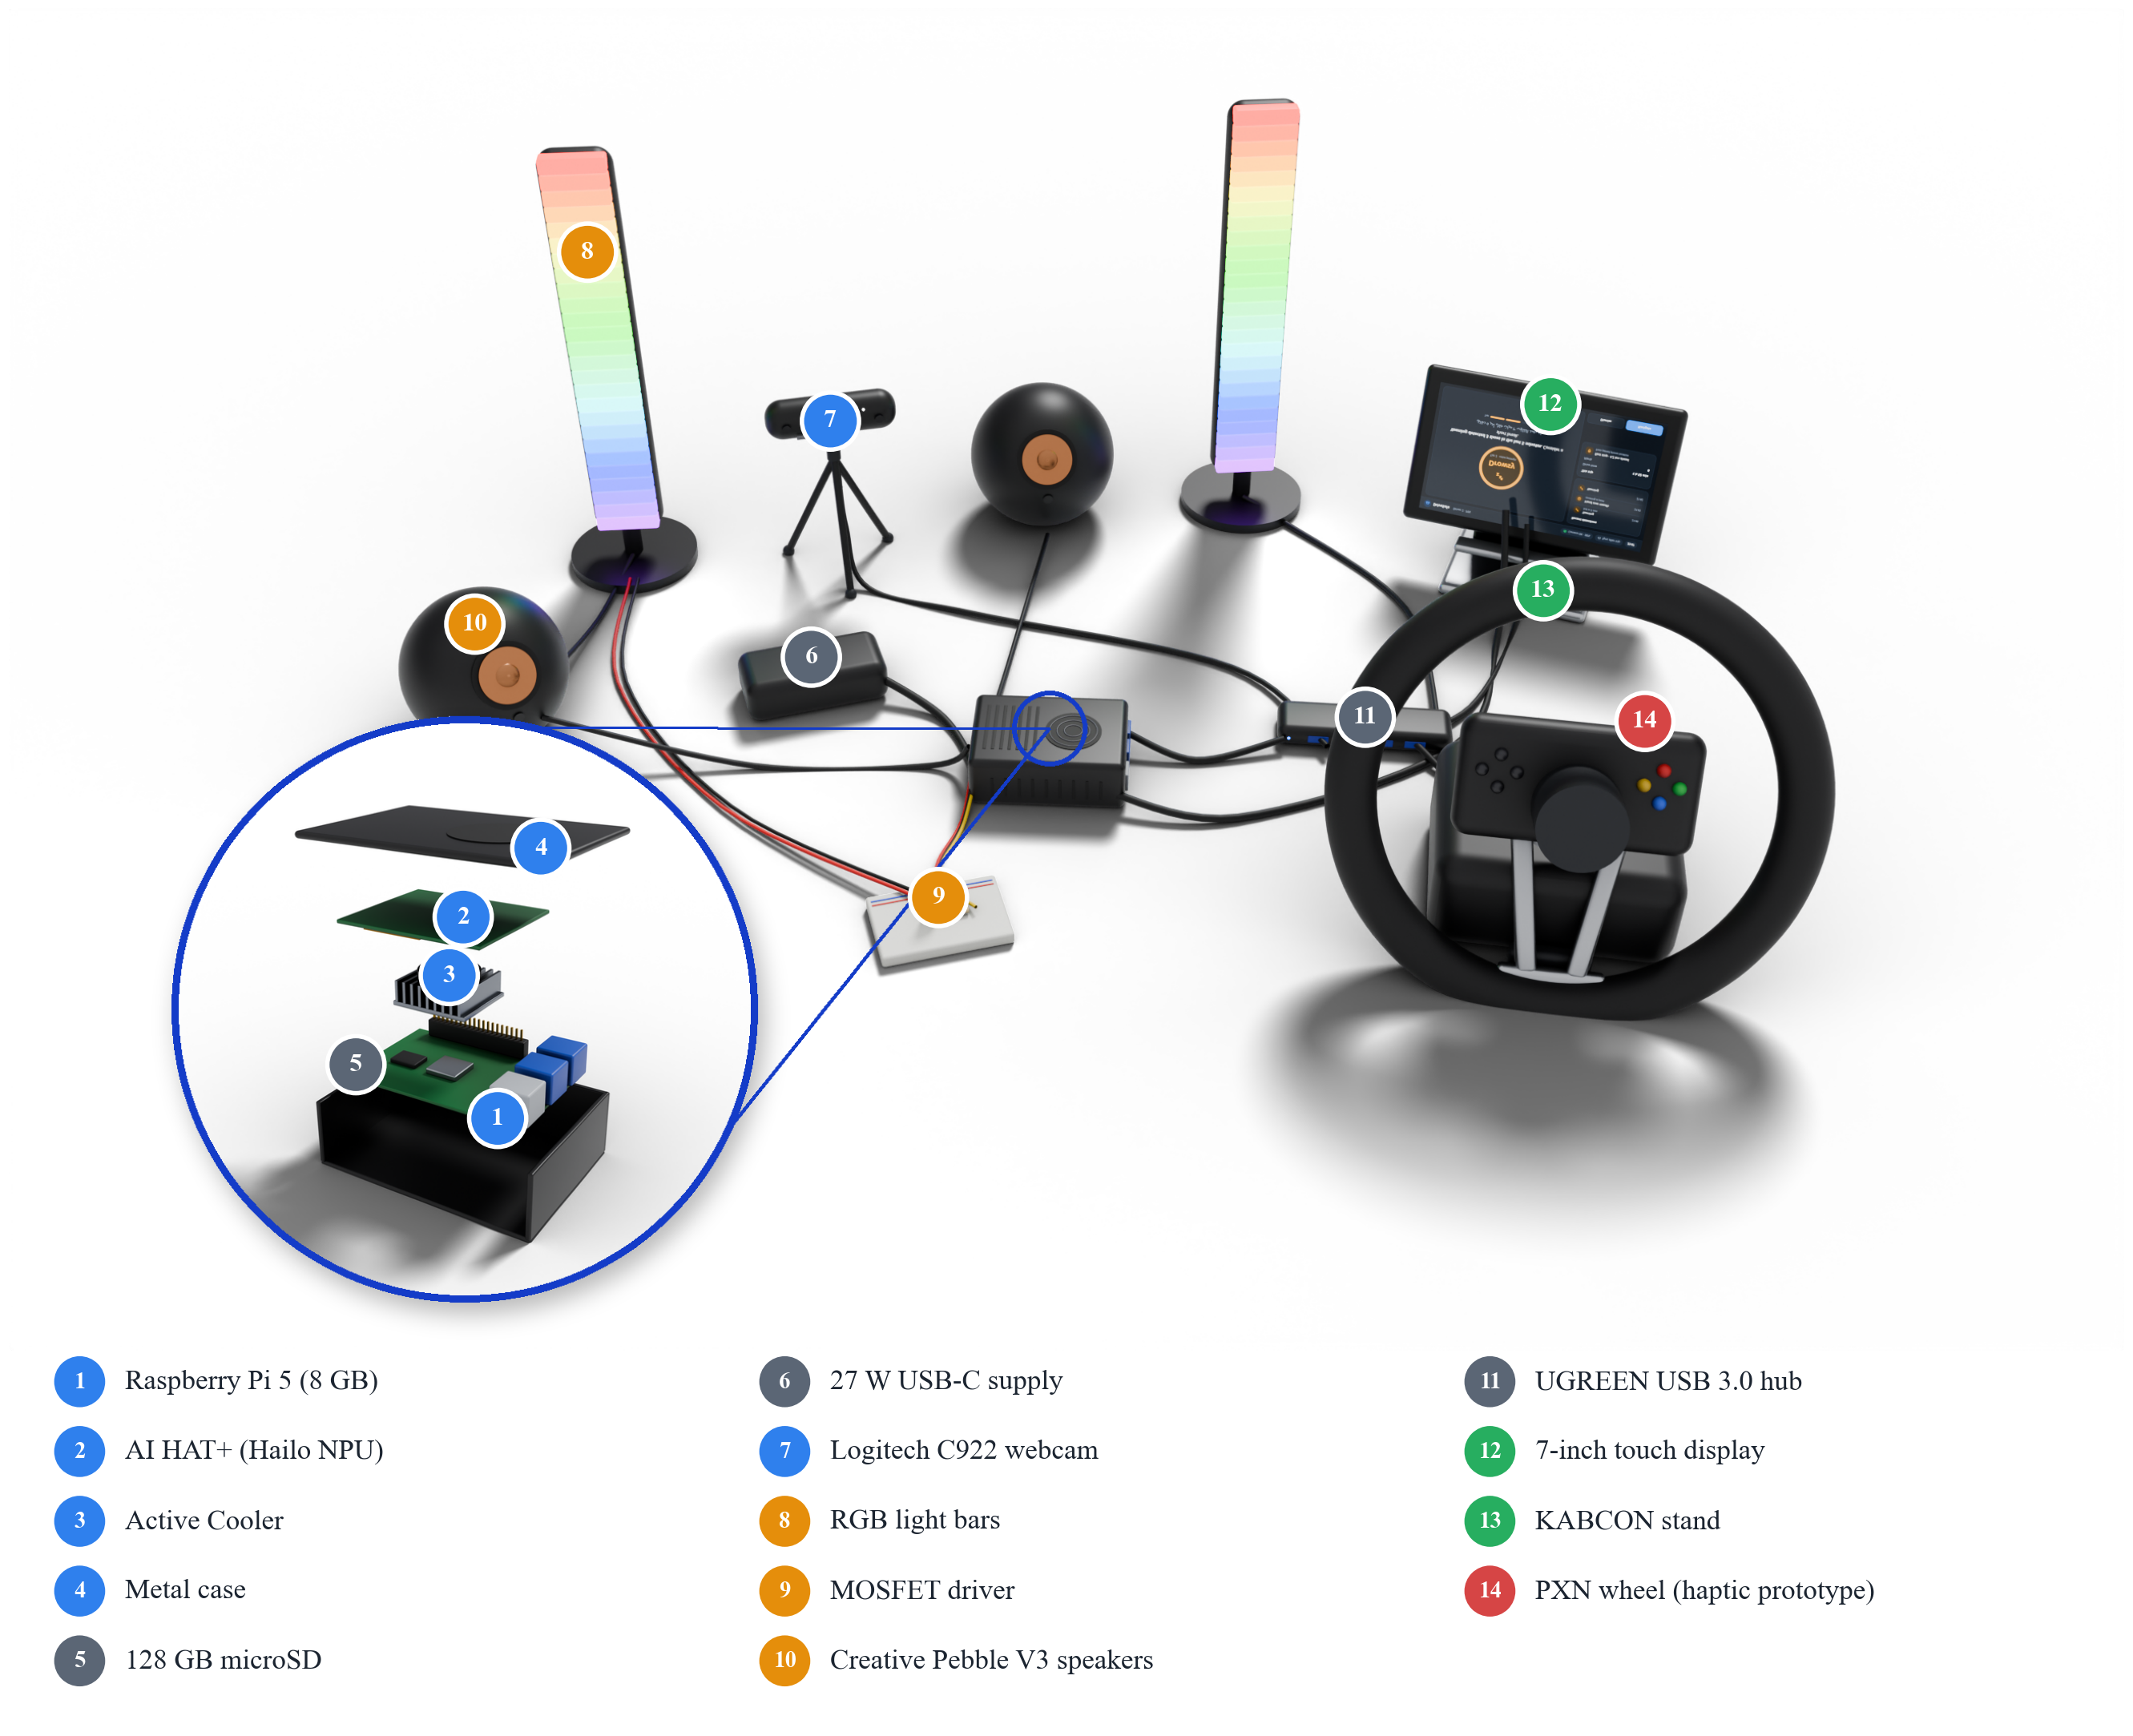
\includegraphics[width=\linewidth]{Figures/bench_3d.png}
  \caption{SDP~2 hardware bench with all purchased parts and a magnifier showing the stack inside the case (Blender render)}
  \label{fig:ch4-bench}
\end{figure}

\begin{figure}[htbp]
  \centering
  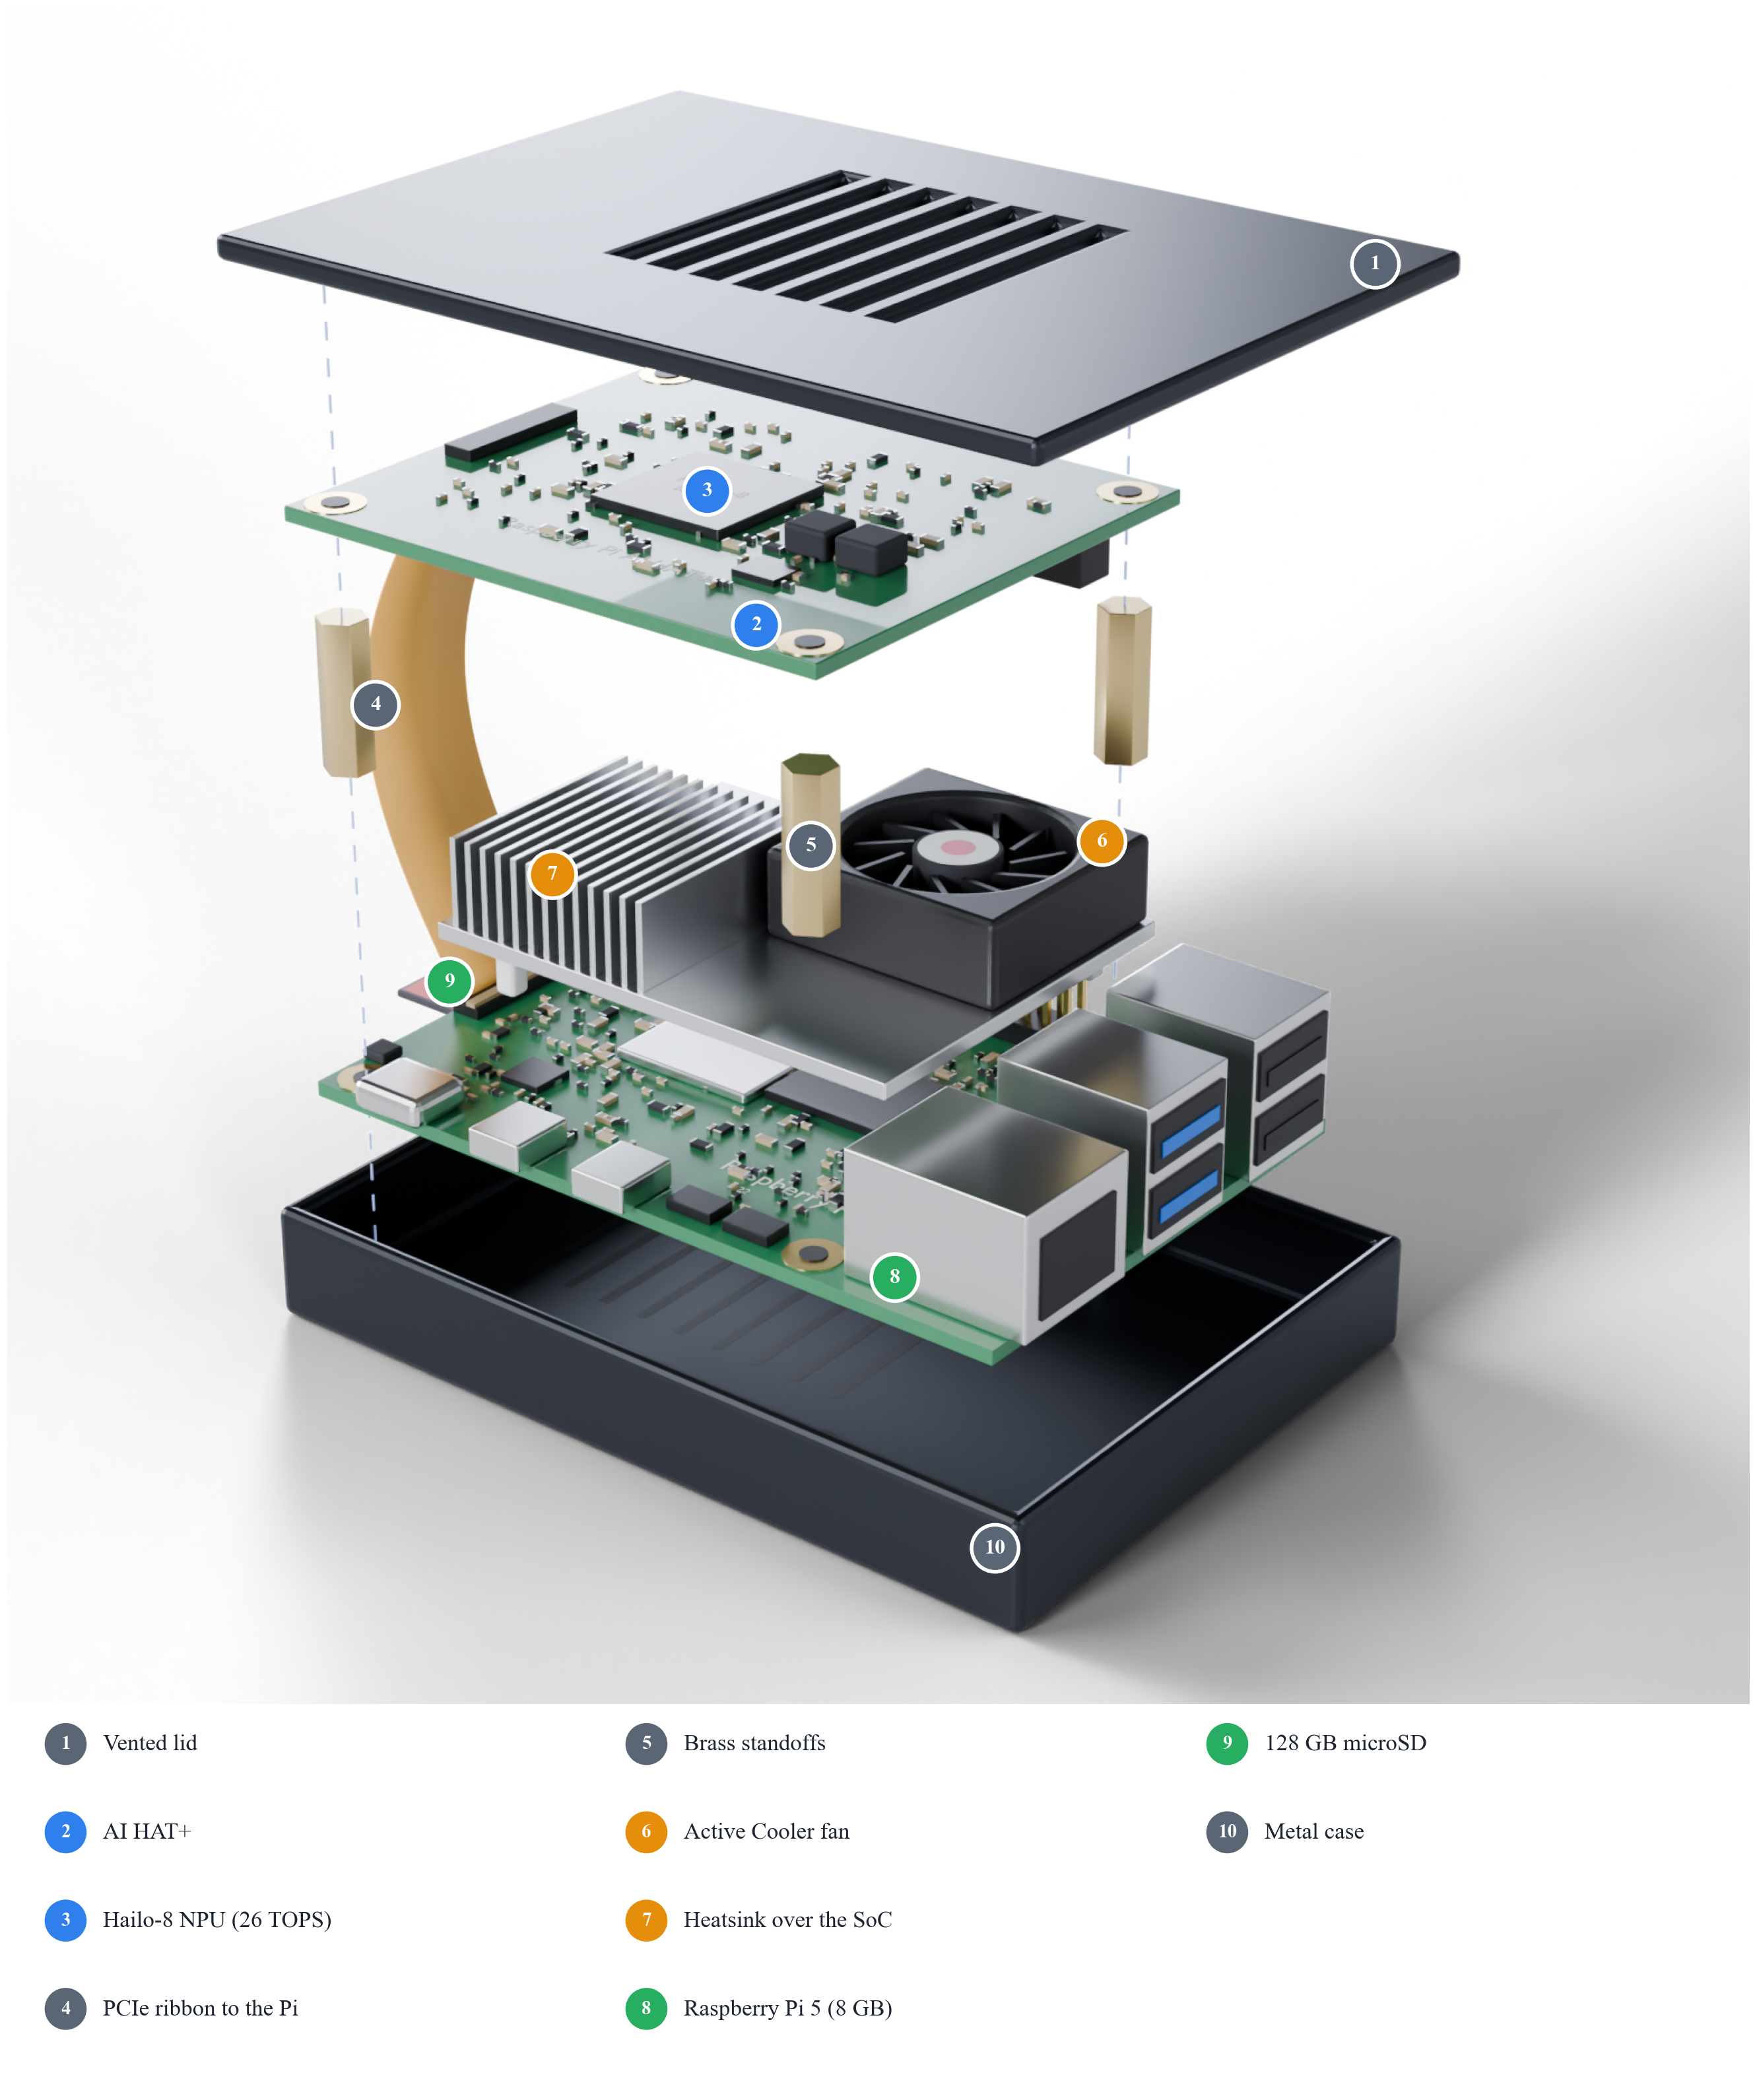
\includegraphics[width=0.6\linewidth]{Figures/edge_unit.png}
  \caption{Edge unit, exploded from the case to the lid (Blender render)}
  \label{fig:ch4-edge}
\end{figure}

\subsubsection{Circuit and wiring diagram with all connections}

A \gls{gpio} pin cannot supply the current the light bar needs, so a logic-level N-channel \gls{mosfet} switches the ground side of the bar. \gls{gpio}18 (pin 12) drives the gate through a 220\,$\Omega$ resistor, while a 10\,k$\Omega$ pull-down keeps the bar off as the Pi boots. The bar takes 5 V from pin 2, and the source joins the common ground at pin 6. All other parts use standard \gls{usb}, micro-\gls{hdmi}, \gls{pcie} and \gls{usb}-C connectors. Figure \ref{fig:ch4-06} shows the wiring alongside its schematic.

\begin{figure}[htbp]
  \centering
  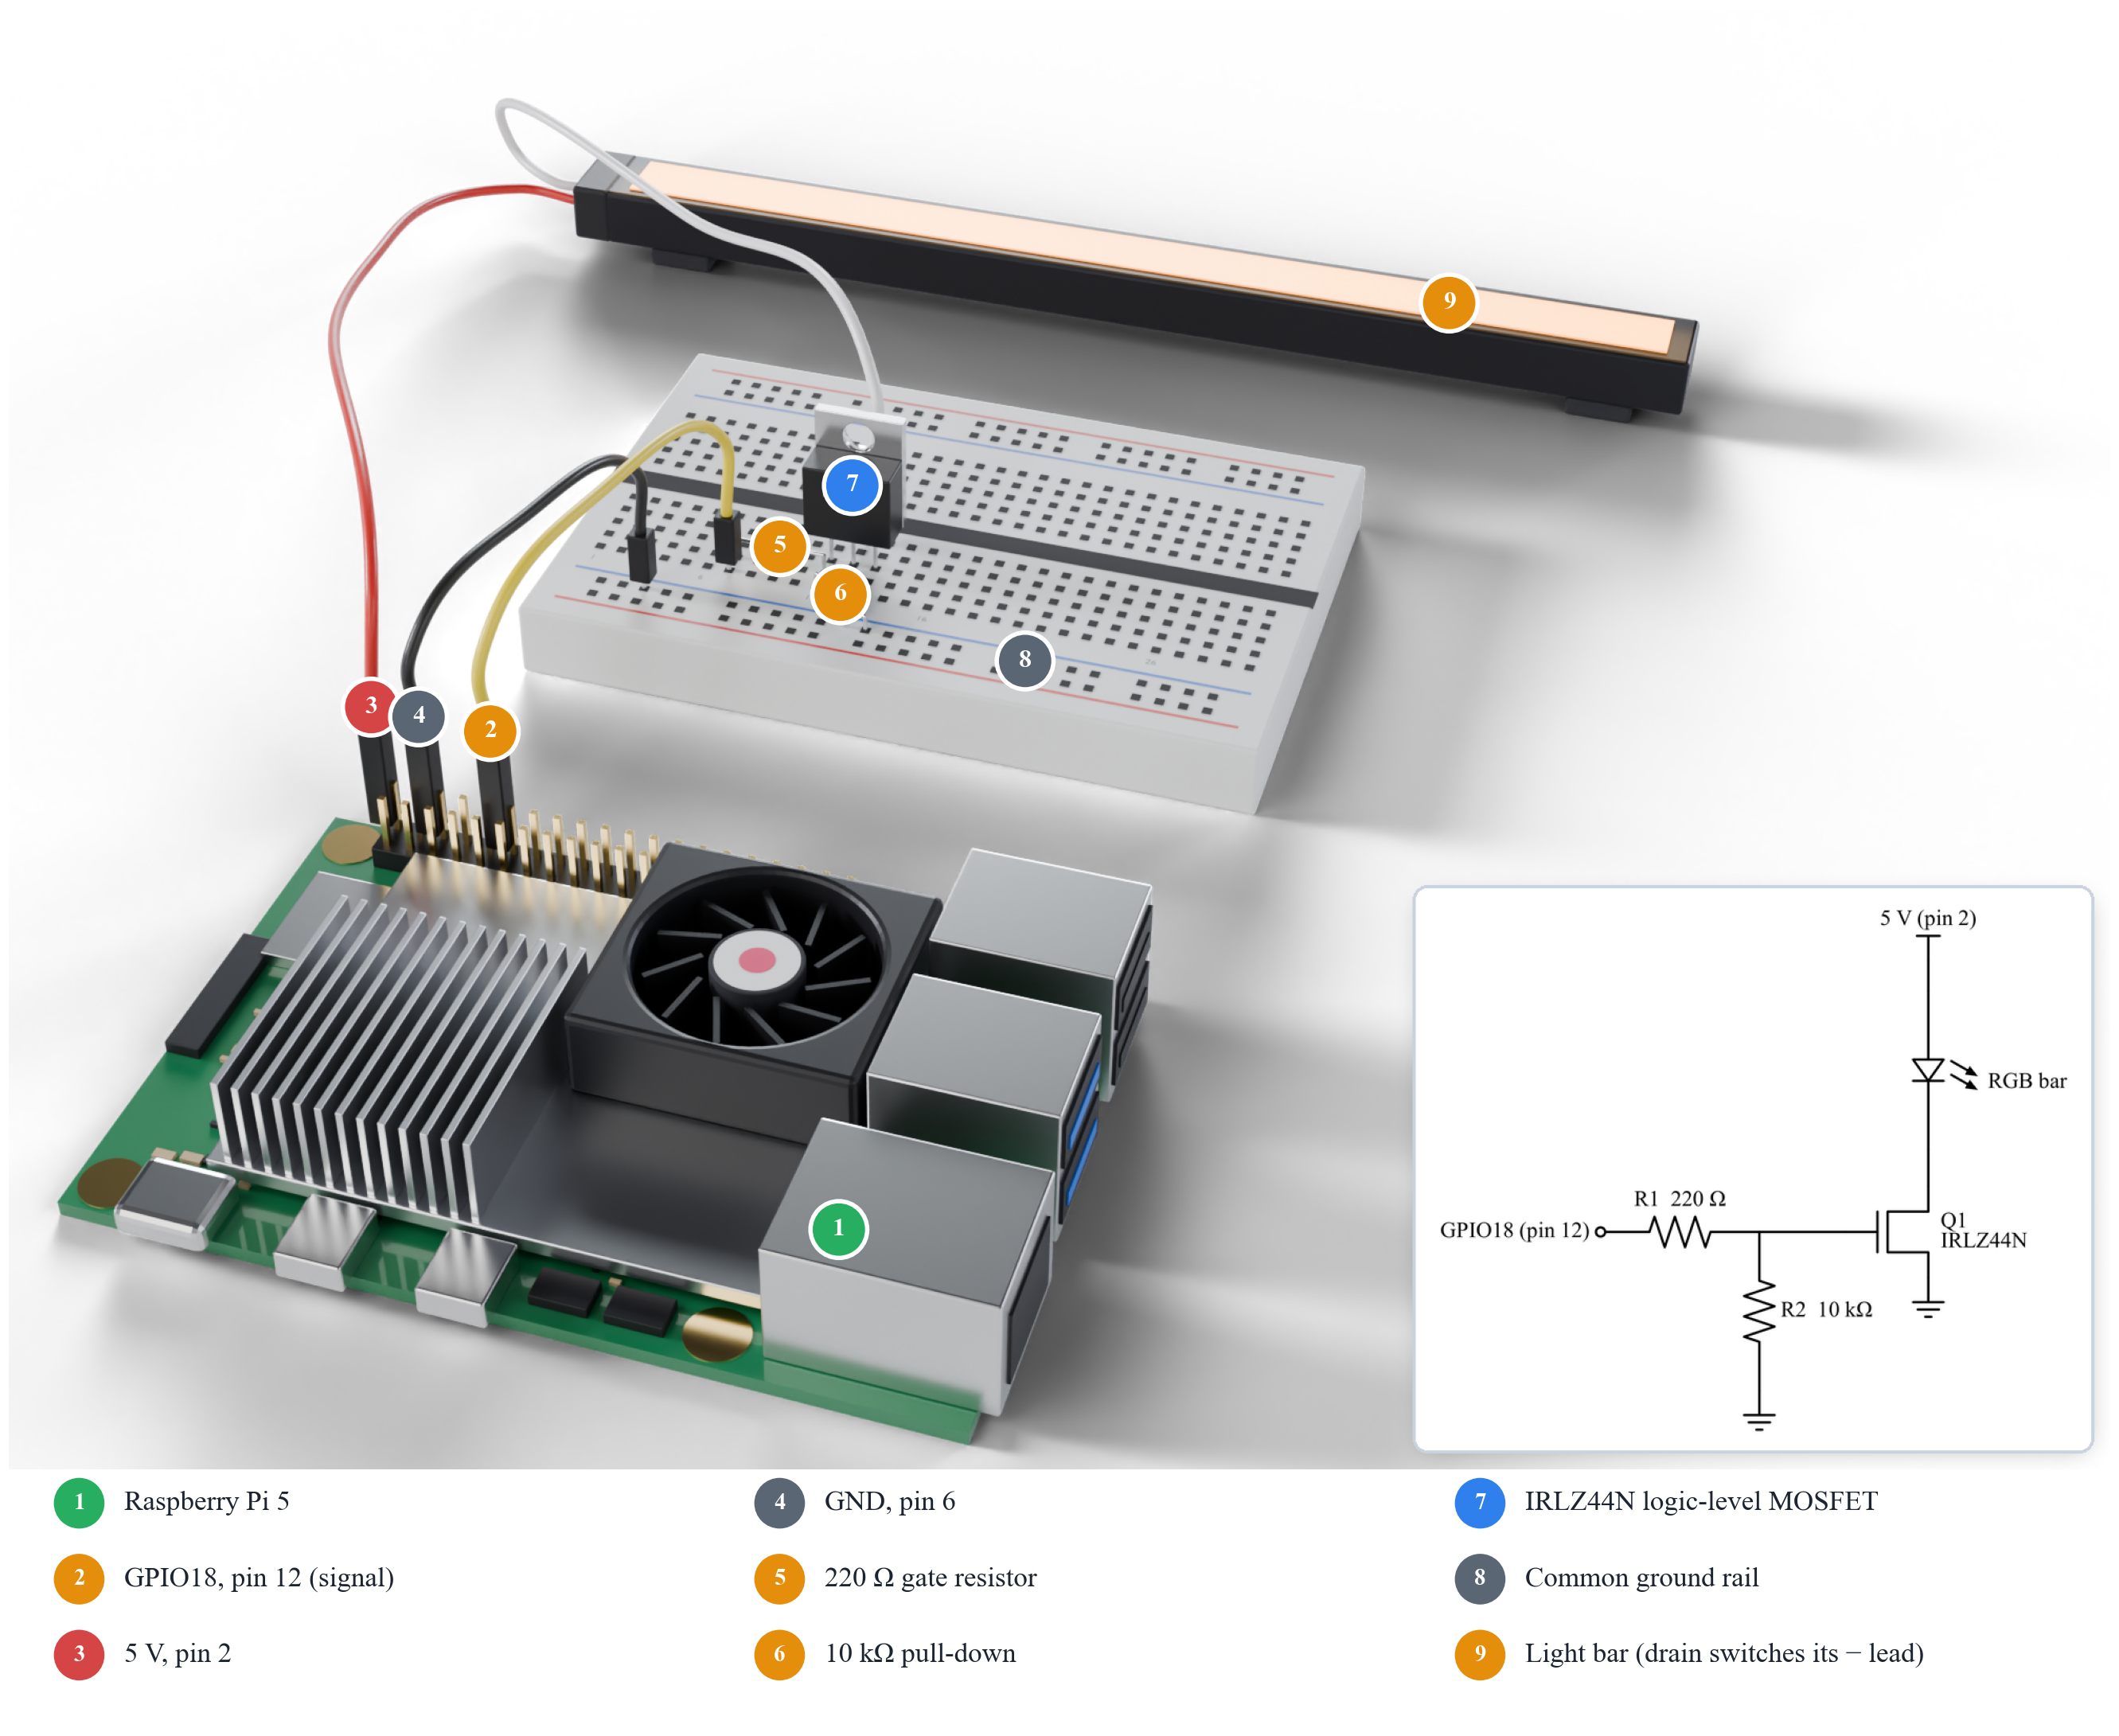
\includegraphics[width=\linewidth]{Figures/wiring_real.png}
  \caption{Light-bar driver on the breadboard, with its schematic (Blender render)}
  \label{fig:ch4-06}
\end{figure}

\subsubsection{Power chain and power budget}
\label{sec:power}

All loads share the 5.1 V, 5 A rail of the official 27 W supply, with the \gls{usb} ports sharing 1.6 A \cite{r50}. Table \ref{tab:ch4-13} estimates a typical draw of 3.25 A (16.3 W), leaving about 9 W of margin. In the worst case, with every load at its peak, the draw slightly exceeds both 5 A and the \gls{usb} limit, so we cap speaker volume and light brightness in software, powering the hub separately should bench tests confirm the issue. The demonstration rig runs from mains, while an in-car version would use a 12 V PD adapter rated for ISO 7637-2 transients \cite{r59}.

\begin{table}[htbp]
\centering
\caption{Estimated power budget (5 V rail), to be measured in SDP~2}
\label{tab:ch4-13}
\footnotesize
\setlength{\tabcolsep}{3pt}
\renewcommand{\arraystretch}{1.15}
\begin{tabular}{|p{0.370\linewidth}|p{0.110\linewidth}|p{0.140\linewidth}|p{0.120\linewidth}|p{0.140\linewidth}|}
\hline
\textbf{Component} & \textbf{Voltage} & \textbf{Typical A} & \textbf{Peak A} & \textbf{Watts (typ.)} \\
\hline
Raspberry Pi 5 with active cooler & 5 V & 1.20 & 2.00 & 6.0 \\
\hline
AI HAT+ (Hailo \gls{npu}) & 5 V & 0.50 & 0.60 & 2.5 \\
\hline
Logitech C922 (\gls{usb}) & 5 V & 0.25 & 0.50 & 1.3 \\
\hline
Creative Pebble V3 (\gls{usb}) & 5 V & 0.40 & 1.00 & 2.0 \\
\hline
7-inch display and touch & 5 V & 0.50 & 0.80 & 2.5 \\
\hline
\gls{rgb} light bar via \gls{mosfet} & 5 V & 0.30 & 0.60 & 1.5 \\
\hline
\gls{usb} hub and PXN wheel & 5 V & 0.10 & 0.30 & 0.5 \\
\hline
\textbf{Total} & 5 V & \textbf{3.25} & \textbf{5.80} & \textbf{16.3} \\
\hline
\end{tabular}
\end{table}

\subsubsection{Target in-car placement}

In a vehicle, which remains the target of the product beyond SDP~2, the camera sits on the dashboard above the steering column, capturing the face and both hands of the driver. The light bar runs along the dashboard edge within peripheral vision, the display sits by the centre vents, within reach but outside the line of sight, and the edge unit rests on the centre console, where it is shaded and ventilated. Figure \ref{fig:ch4-09} shows this placement next to a real view from one of our pilot sessions, while Section \ref{sec:pilot} explains why the camera does not go below the wheel.

\begin{figure}[htbp]
  \centering
  \begin{subfigure}[b]{0.655\linewidth}\centering
    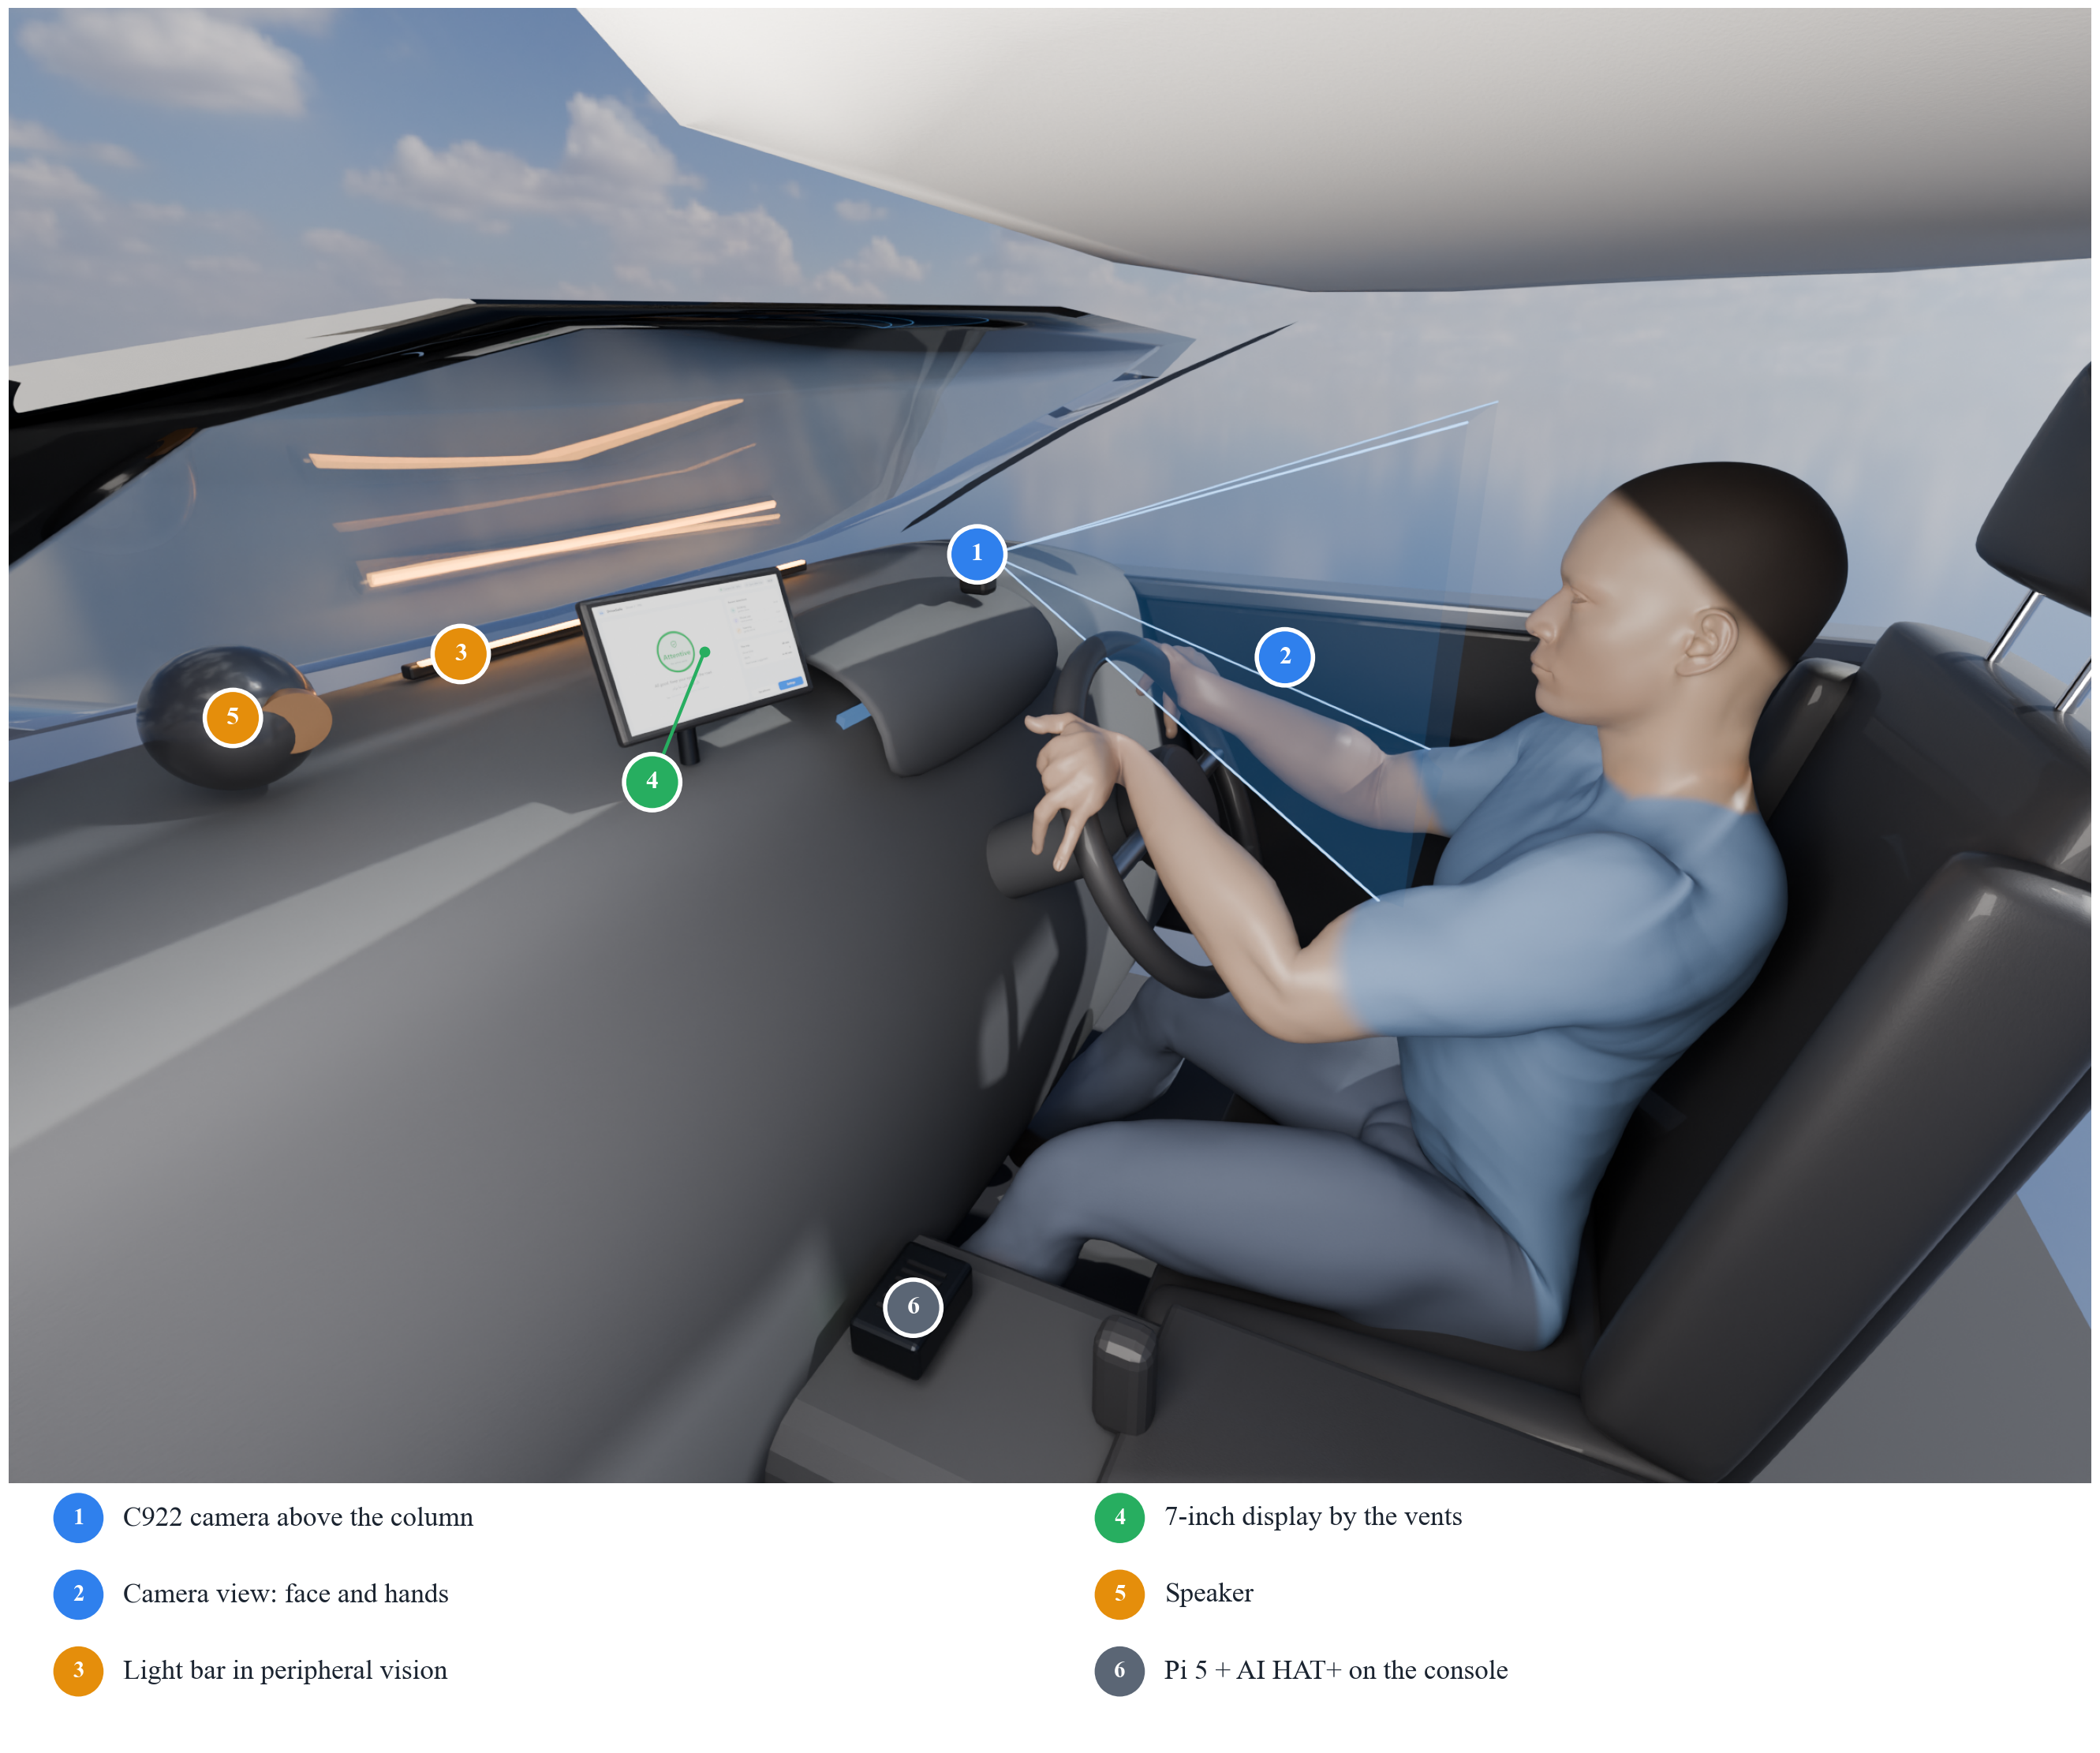
\includegraphics[width=\linewidth]{Figures/cabin_real.png}
    \caption{Target in-car placement (Blender render, driver from the Blender Studio CC0 base meshes)}
  \end{subfigure}\hfill
  \begin{subfigure}[b]{0.325\linewidth}\centering
    
\includegraphics[width=\linewidth]{Figures/pilot/pilot_dash_view.jpg}
    \caption{Real view from a dash mount (pilot session C3)}
  \end{subfigure}
  \caption{Target in-car placement and what the camera sees}
  \label{fig:ch4-09}
\end{figure}

\subsection{Software design in detail}
\subsubsection{Software architecture and module hierarchy}

The software consists of small Python modules connected by queues (Figure \ref{fig:ch4-10}). A capture thread passes on only the latest frame, so a slow stage never builds a backlog. The detector runs in its own thread on the \gls{npu}, the filter, decision logic and alerts share the main loop, and the logger, uploader, display server and eye module run in their own threads. Each Desired feature plugs into this loop without changing it, allowing features to be added or removed one at a time.

\begin{figure}[htbp]
  \centering
  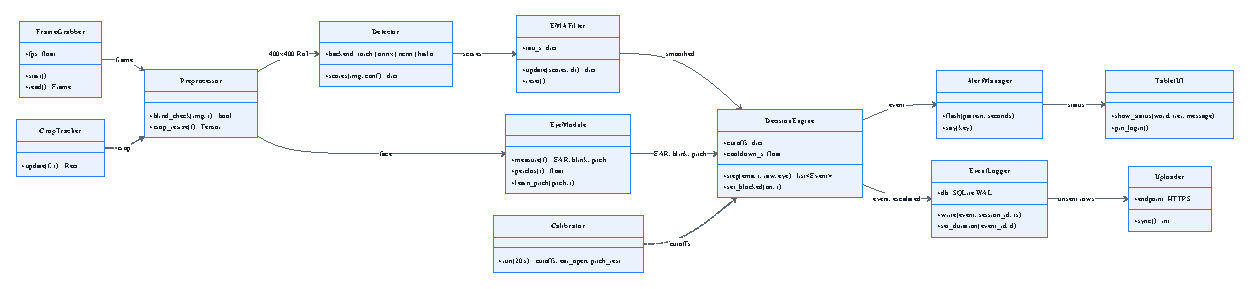
\includegraphics[width=\linewidth]{Figures/uml_class.pdf}
  \caption{UML class diagram of the main software modules}
  \label{fig:ch4-10}
\end{figure}

\subsubsection{Training and optimising the detector}

\gls{yolo}11n is fine-tuned from its \gls{coco} weights on the subject-disjoint training split at an image size of 640, with augmentation for lighting, small rotations and horizontal flips. The validation split is used for early stopping and for choosing cutoffs, while the test split is touched only once, at the very end. Table \ref{tab:ch4-14} lists the settings.

Compression follows a fixed order: fine-tune, prune in 10\% steps, fine-tune again, quantize to \gls{int} with the Hailo Dataflow Compiler, and finally benchmark on the Pi. A variant is acceptable when recall drops by no more than 2 points and \gls{map}$_{50}$ by no more than 3 points against the FP32 model, and the fastest acceptable variant is deployed (Table \ref{tab:ch4-14}).

\begin{table}[htbp]
\centering
\caption{Training settings and compression configurations}
\label{tab:ch4-14}
\footnotesize
\setlength{\tabcolsep}{3pt}
\renewcommand{\arraystretch}{1.15}
\begin{tabular}{|p{0.200\linewidth}|p{0.330\linewidth}|p{0.400\linewidth}|}
\hline
\textbf{Stage} & \textbf{Setting} & \textbf{Value} \\
\hline
Fine-tuning & Initial weights, image size & \gls{coco} \gls{yolo}11n, 640 \\
\hline
Fine-tuning & Augmentation & Brightness and contrast, hue, $\pm$10$^\circ$ rotation, horizontal flip, mosaic \\
\hline
Fine-tuning & Epochs, early stopping & Up to 150, patience 30 on validation \gls{map}$_{50}$ \\
\hline
Pruning & Structured, by channel L1 norm & 10\%, 20\%, 30\% then fine-tune \\
\hline
Quantization & Methods compared & Hailo \gls{int} (\gls{ptq}), \gls{onnx} FP16 and \gls{int}, NCNN \gls{int} \\
\hline
Selection & Acceptable & Recall drop $\le$ 2 points, \gls{map}$_{50}$ drop $\le$ 3 points \\
\hline
\end{tabular}
\end{table}

\subsubsection{Region-of-interest crop}
\label{sec:roi}

Each frame is first cut to a 640$\times$640 square, from which a fixed 400$\times$400 \gls{roi} at $x \in [140, 540]$, $y \in [120, 520]$ is extracted and resized to the model input (Figure \ref{fig:ch4-roi}). Since the driver occupies a predictable region of an in-cabin view, the \gls{roi} keeps the face and hands, discards 61\% of the pixels, and enlarges small cues: at a 320-pixel input, the median yawning box grows from 35 to 55 pixels \cite{rs3}. Detections are then mapped back to the full frame. The cost falls on the edges of the frame, as drivers tend to hold a phone toward the door, so 9.3\% of test phone-use boxes in DMD leave the window \cite{rs3}. Crop tracking (Table \ref{tab:ch4-desired}) moves the window with the face to reduce this loss.

\begin{figure}[htbp]
  \centering
  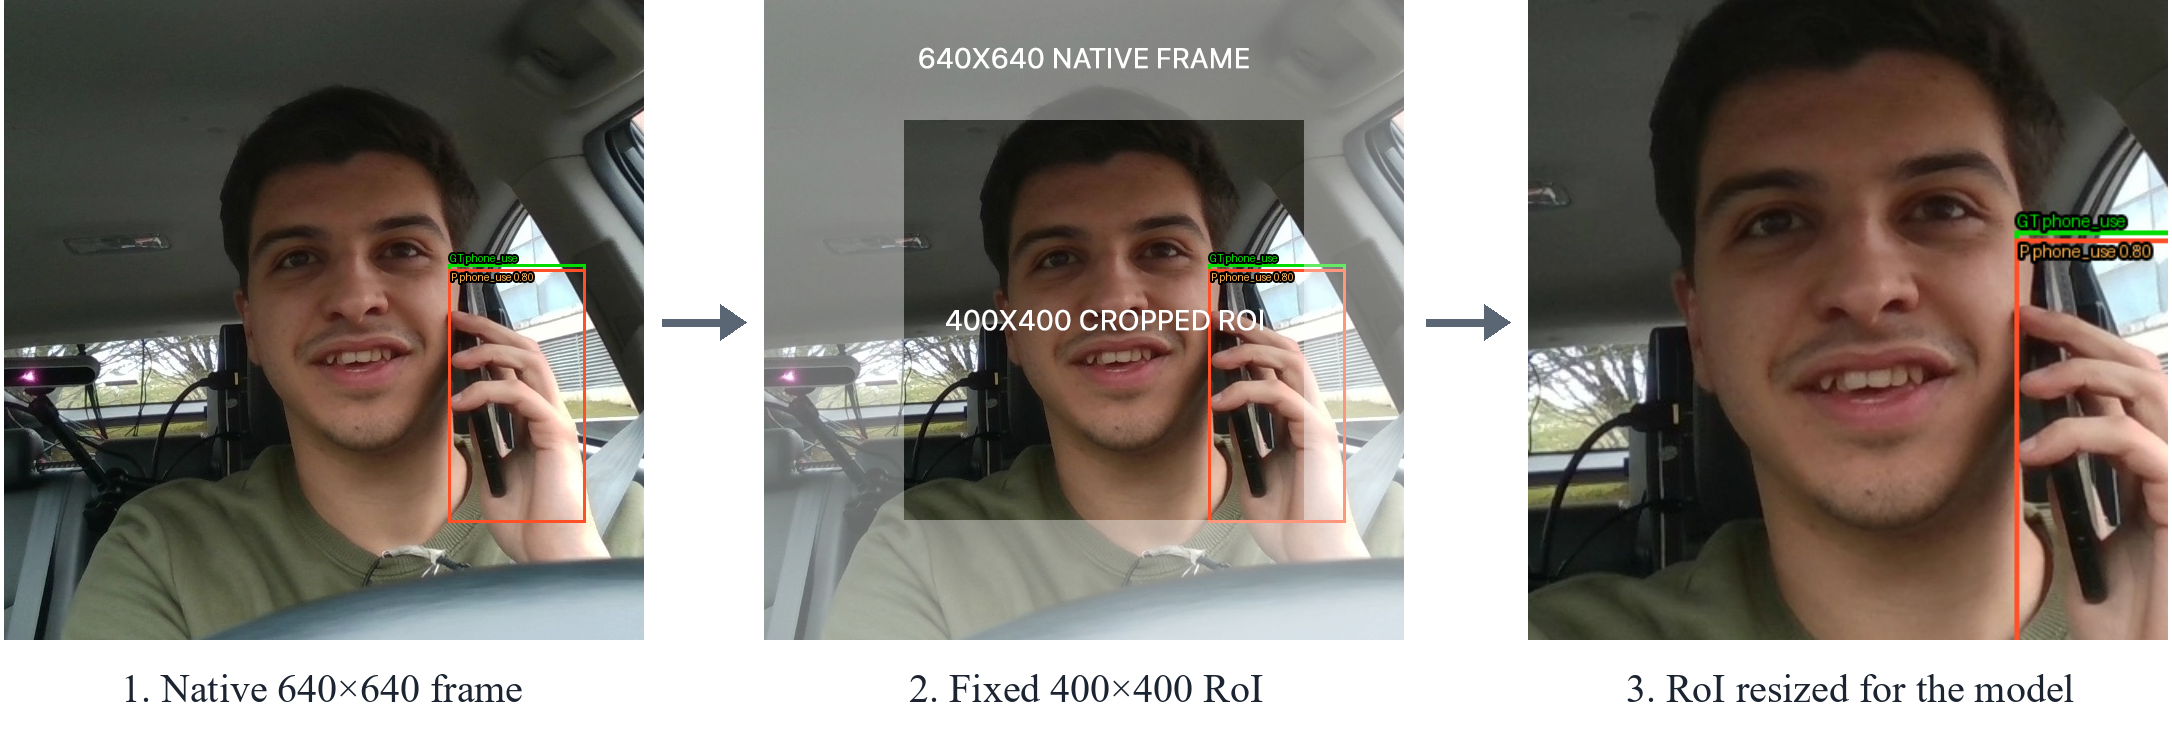
\includegraphics[width=\linewidth]{Figures/crop_roi.png}
  \caption{Static \glsentryshort{roi} crop on a DMD frame: the phone box (ground truth in green, prediction in red) stays inside the window and gets larger (from \cite{rs3})}
  \label{fig:ch4-roi}
\end{figure}

\subsubsection{Temporal filtering with EMA}

Each class has its own $\tau$: 0.6\,s for yawning and hand-over-mouth, which are short and distinct, and 1.0\,s for drinking and phone use, which last longer and have more look-alikes. The filter restarts from zero after boot and after a camera-blocked period, ensuring old evidence never carries over. Since $\alpha$ is computed from the measured $\Delta t$ in Equation \ref{eq:ema}, the filter is tested by replaying the same clip at 10, 15 and 30 \gls{fps} and checking that confirmation times agree within one frame.

\subsubsection{Alert decision logic: class-specific alerts, cool-down, escalation and suppression}
\label{sec:decision}

Each class has a default cutoff and, after calibration, a per-driver cutoff kept between the default and 0.85. A cue is confirmed once its smoothed score stays above the cutoff for the class confirmation time. When the cue ends, the class is muted for a 30\,s cool-down, and any cue inside the cool-down is logged as tier 0 without playing an alert. Counting from the end of the cue allows Tiers 2 and 3 to fire while a cue persists, whereas the eye-closure alarm has no cool-down, being the most dangerous case. Each class has its own light pattern and sound, always below 3 flashes per second. We designed three alarm sounds in \gls{matlab}: a gentle 1.5\,s chime for distractions, a 3\,s 350\,\gls{hz} buzz for yawning, and a 10\,s emergency alarm reserved for risky driving. Table \ref{tab:ch4-15} lists the per-class settings.

Alerts escalate in three tiers while the risk persists (Figure \ref{fig:ch4-14}). Tier 1 is the class chime with a short light pulse. Tier 2 adds an explained voice prompt, after 5\,s or after three cues within 5 minutes. Tier 3 is the emergency alarm with the full light pattern, after 10\,s, or immediately when the eyes stay closed for 1.5\,s (3\,s with the head down). The \gls{perclos} warning acts as a gentle Tier 2 prompt. Every voice message names what was detected and for how long or how often, in both English and Arabic. Since a single \gls{mosfet} can flash the bar but not change its colour, the colours in Table \ref{tab:ch4-15} appear on the display instead.

Mirror checks never trigger an alert, as head orientation is not one of our classes. Suppression while reversing, at red lights or in heavy traffic requires vehicle signals, and therefore remains a Future item.

\begin{figure}[htbp]
  \centering
  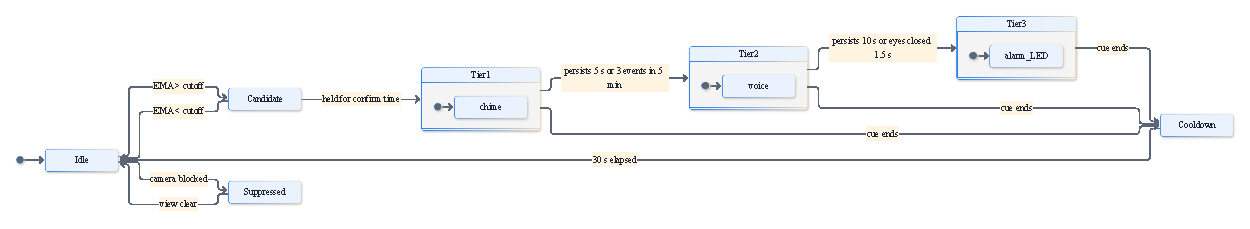
\includegraphics[width=\linewidth]{Figures/uml_state.pdf}
  \caption{Alert state machine with the three tiers, cool-down and suppression}
  \label{fig:ch4-14}
\end{figure}

\begin{table}[htbp]
\centering
\caption{Per-class alert settings}
\label{tab:ch4-15}
\footnotesize
\setlength{\tabcolsep}{3pt}
\renewcommand{\arraystretch}{1.15}
\begin{tabular}{|p{0.140\linewidth}|p{0.090\linewidth}|p{0.060\linewidth}|p{0.090\linewidth}|p{0.170\linewidth}|p{0.360\linewidth}|}
\hline
\textbf{Class} & \textbf{Default cutoff} & \textbf{$\tau$ (s)} & \textbf{Confirm (s)} & \textbf{Light pattern} & \textbf{Voice message (Tier 2)} \\
\hline
Yawning & 0.50 & 0.6 & 1.0 & Amber, 1 Hz pulse & ``Yawning detected 3 times in 5 minutes. Consider a short break.'' \\
\hline
Hand-over-mouth & 0.50 & 0.6 & 1.0 & Amber, 1 Hz pulse & ``Hand over mouth detected for 5 seconds. You seem tired. Consider a short break.'' \\
\hline
Drinking & 0.55 & 1.0 & 1.5 & Teal, single pulse & ``Drinking detected. Keep your eyes on the road.'' \\
\hline
Phone use & 0.55 & 1.0 & 2.0 & Purple, 2 Hz & ``Phone use detected for 5 seconds. Please put the phone down.'' \\
\hline
Eyes closed & 0.50 $\times$ \gls{ear}$_\text{open}$ and blink score $>$ 0.50 & -- & 1.5 (3.0 head down) & Red, 3 Hz & ``Eyes closed for 1.5 seconds. Pull over safely.'' (Tier 3) \\
\hline
\end{tabular}
\end{table}

\subsubsection{New-driver calibration algorithm}
\label{sec:calib}

During a 20\,s window, guided by prompts on the display, the driver sits normally while the detector runs at a confidence of 0.05. Since the driver performs no cue in this window, every detection within it is treated as a false alarm. For each class $c$, the cutoff becomes
\begin{equation}
\theta_c = \min\!\left(\max\!\left(P_{99}(\text{scores}_c) + 0.05,\; \theta_c^{\text{default}}\right),\; 0.85\right).
\end{equation}
We define ``many detections'' as more than 10\% of the 600 baseline frames scoring above the default cutoff in any class, indicating that the driver moved or performed a cue, in which case the defaults are kept and the driver is asked to redo the baseline. The same window also stores the driver's open-eye \gls{ear} and rest head pitch. Figure \ref{fig:ch4-15} shows two example drivers and the flow.

\begin{figure}[htbp]
\centering
\begin{subfigure}[b]{\linewidth}
\centering
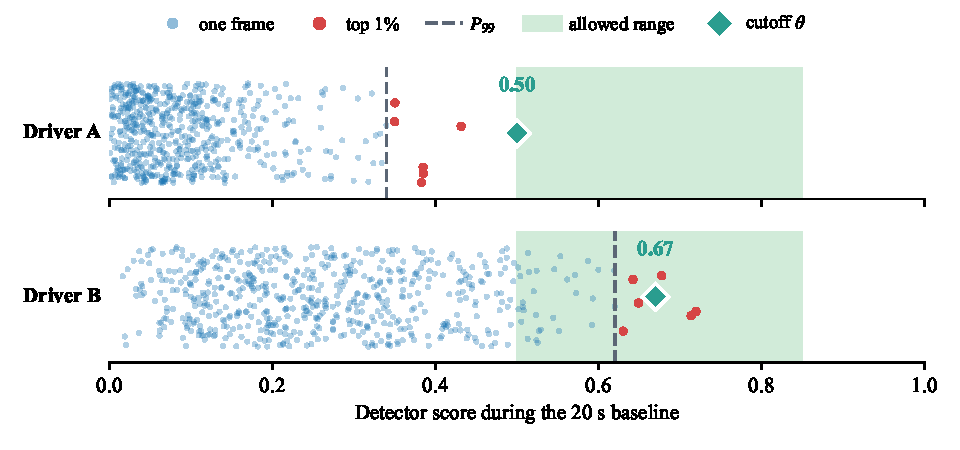
\includegraphics[width=\linewidth]{Figures/calib_strip.pdf}
\caption{Two example drivers: the cutoff is $P_{99}$ plus 0.05, kept inside the allowed range (illustrative)}
\end{subfigure}\\[3mm]
\begin{subfigure}[b]{\linewidth}
\centering
\resizebox{\linewidth}{!}{\begin{tikzpicture}[node distance=6mm and 8mm]
  \fterm{n}{sbblue}{New driver}{}
  \fcard{p}{sbblue}{\faUser}{Prompt: sit normally, eyes on the road}{right=of n}
  \fcard{r}{sbblue}{\faStopwatch}{Detector at 0.05 for 20\,s (600 frames)}{right=of p}
  \fdec{q}{sbblue}{Over 10\% of frames above default?}{right=of r}
  \fcard{k}{sbred}{\faRedo}{Keep defaults, ask to redo}{above=10mm of q}
  \fcard{s}{sbblue}{\faPercent}{Per class: $P_{99}$ + 0.05}{below=10mm of q}
  \fcard{c}{sbblue}{\faCompress}{Clamp between default and 0.85}{left=of s}
  \fcard{e}{sbblue}{\faEye}{Store open-eye \gls{ear}}{left=of c}
  \fterm{v}{sbgreen}{Save cutoffs}{left=of e}
  \draw[farr] (n) -- (p); \draw[farr] (p) -- (r); \draw[farr] (r) -- (q);
  \draw[farr] (q) -- node[flab, right]{yes} (k);
  \draw[farr] (k.west) -| (p.north);
  \draw[farr] (q) -- node[flab, right]{no} (s);
  \draw[farr] (s) -- (c); \draw[farr] (c) -- (e); \draw[farr] (e) -- (v);
  \begin{scope}[on background layer]
    \node[freg=sbblue, fit=(n)(k)(s)(v), label={[freglab]north west:New-driver calibration}] {};
  \end{scope}
\end{tikzpicture}
}
\caption{Calibration flow}
\end{subfigure}
\caption{New-driver calibration: the cutoff is the 99th percentile plus 0.05, kept between the default and 0.85}
\label{fig:ch4-15}
\end{figure}

\subsubsection{Desired driver-facing features}

The remaining Desired features each add one small step to the loop of Figure \ref{fig:ch4-12} (Table \ref{tab:ch4-desired}). Two rules apply to all of them: missing data is never treated as good news, so frames without visible eyes are skipped, and the driver never has to touch the display while moving. Figure \ref{fig:ch4-18} shows the eye-closure logic and Figure \ref{fig:ch4-19} the display screens.

\begin{table}[htbp]
\centering
\caption{Desired driver-facing features}
\label{tab:ch4-desired}
\footnotesize
\setlength{\tabcolsep}{3pt}
\renewcommand{\arraystretch}{1.15}
\begin{tabular}{|p{0.150\linewidth}|p{0.430\linewidth}|p{0.250\linewidth}|p{0.090\linewidth}|}
\hline
\textbf{Feature} & \textbf{How it works} & \textbf{Key values} & \textbf{Spec} \\
\hline
Camera-blind check & Mean grey brightness and variance of the Laplacian \cite{r74} per frame. When unclear for 3\,s, it says ``camera blocked'', pauses alerts and logs the period, which feeds the \% of drive time monitored & Brightness $<$ 25 or $>$ 230, variance $<$ 20, tuned on covered-lens and torch tests & FS-17 \\
\hline
Crop tracking & OpenCV YuNet face detector on a 480$\times$270 copy, and the crop centre follows the face through its own \gls{ema} and is clamped at the frame borders. It is kept only if it beats the fixed crop & About 1\,Hz, $\tau = 1$\,s, 640$\times$640 window & FS-18 \\
\hline
Eye closure & MediaPipe Face Mesh \cite{r49} landmarks give the \gls{ear} of both eyes, and an eye is closed below 50\% of the driver's open-eye value with the model's blink score above 0.50. Head pitch more than 8$^\circ$ below the rest value means the driver may only be looking down & 1.5\,s closure $\rightarrow$ Tier 3, 3\,s with the head down, \gls{perclos} $>$ 15\% over 60\,s $\rightarrow$ gentle prompt & FS-20 \\
\hline
Driver display & Full-screen web page served by the Pi: one status (Attentive, Distracted or Drowsy), recent events and trip time, a dark theme after sunset and touch only for \gls{pin}, calibration and settings & 7-inch, 1024$\times$600 & FS-24 \\
\hline
Pre-trip check & Two questions before driving (hours slept, how tired), where a tired answer leads to a suggestion to rest & Two taps & FS-25 \\
\hline
Rest-stop suggestion & Nearest rest stop, fuel station or caf\'e from the paired phone's location (browser geolocation, no \gls{gps} module) through OpenStreetMap \cite{r68}, with the location used once and not stored & Alerts in the last 30 minutes above a threshold & FS-26 \\
\hline
\end{tabular}
\end{table}

\begin{figure}[htbp]
\centering
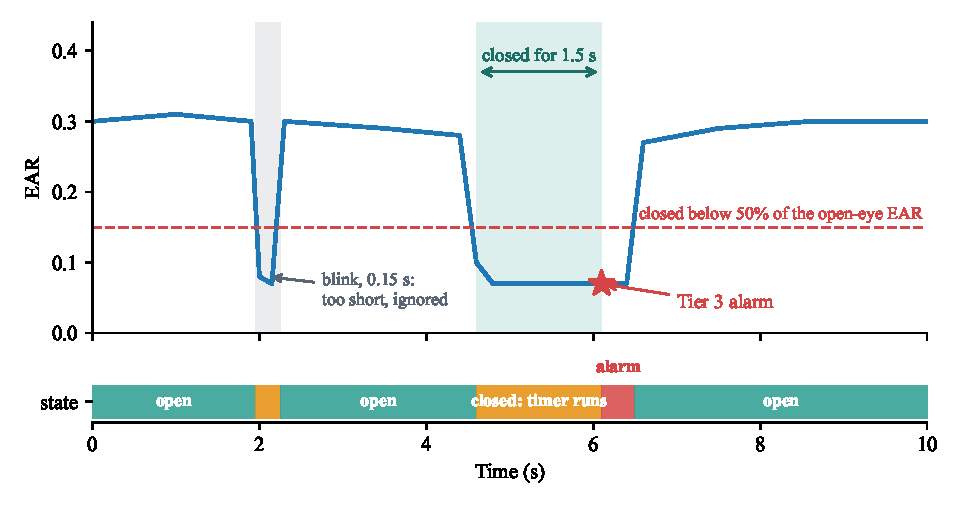
\includegraphics[width=\linewidth]{Figures/eye_closure.pdf}
\caption{Eye-closure rule: a short blink is ignored, eyes closed for 1.5\,s start the Tier 3 alarm (illustrative signal)}
\label{fig:ch4-18}
\end{figure}

\begin{figure}[htbp]
\centering
\begin{subfigure}[t]{0.49\linewidth}\centering
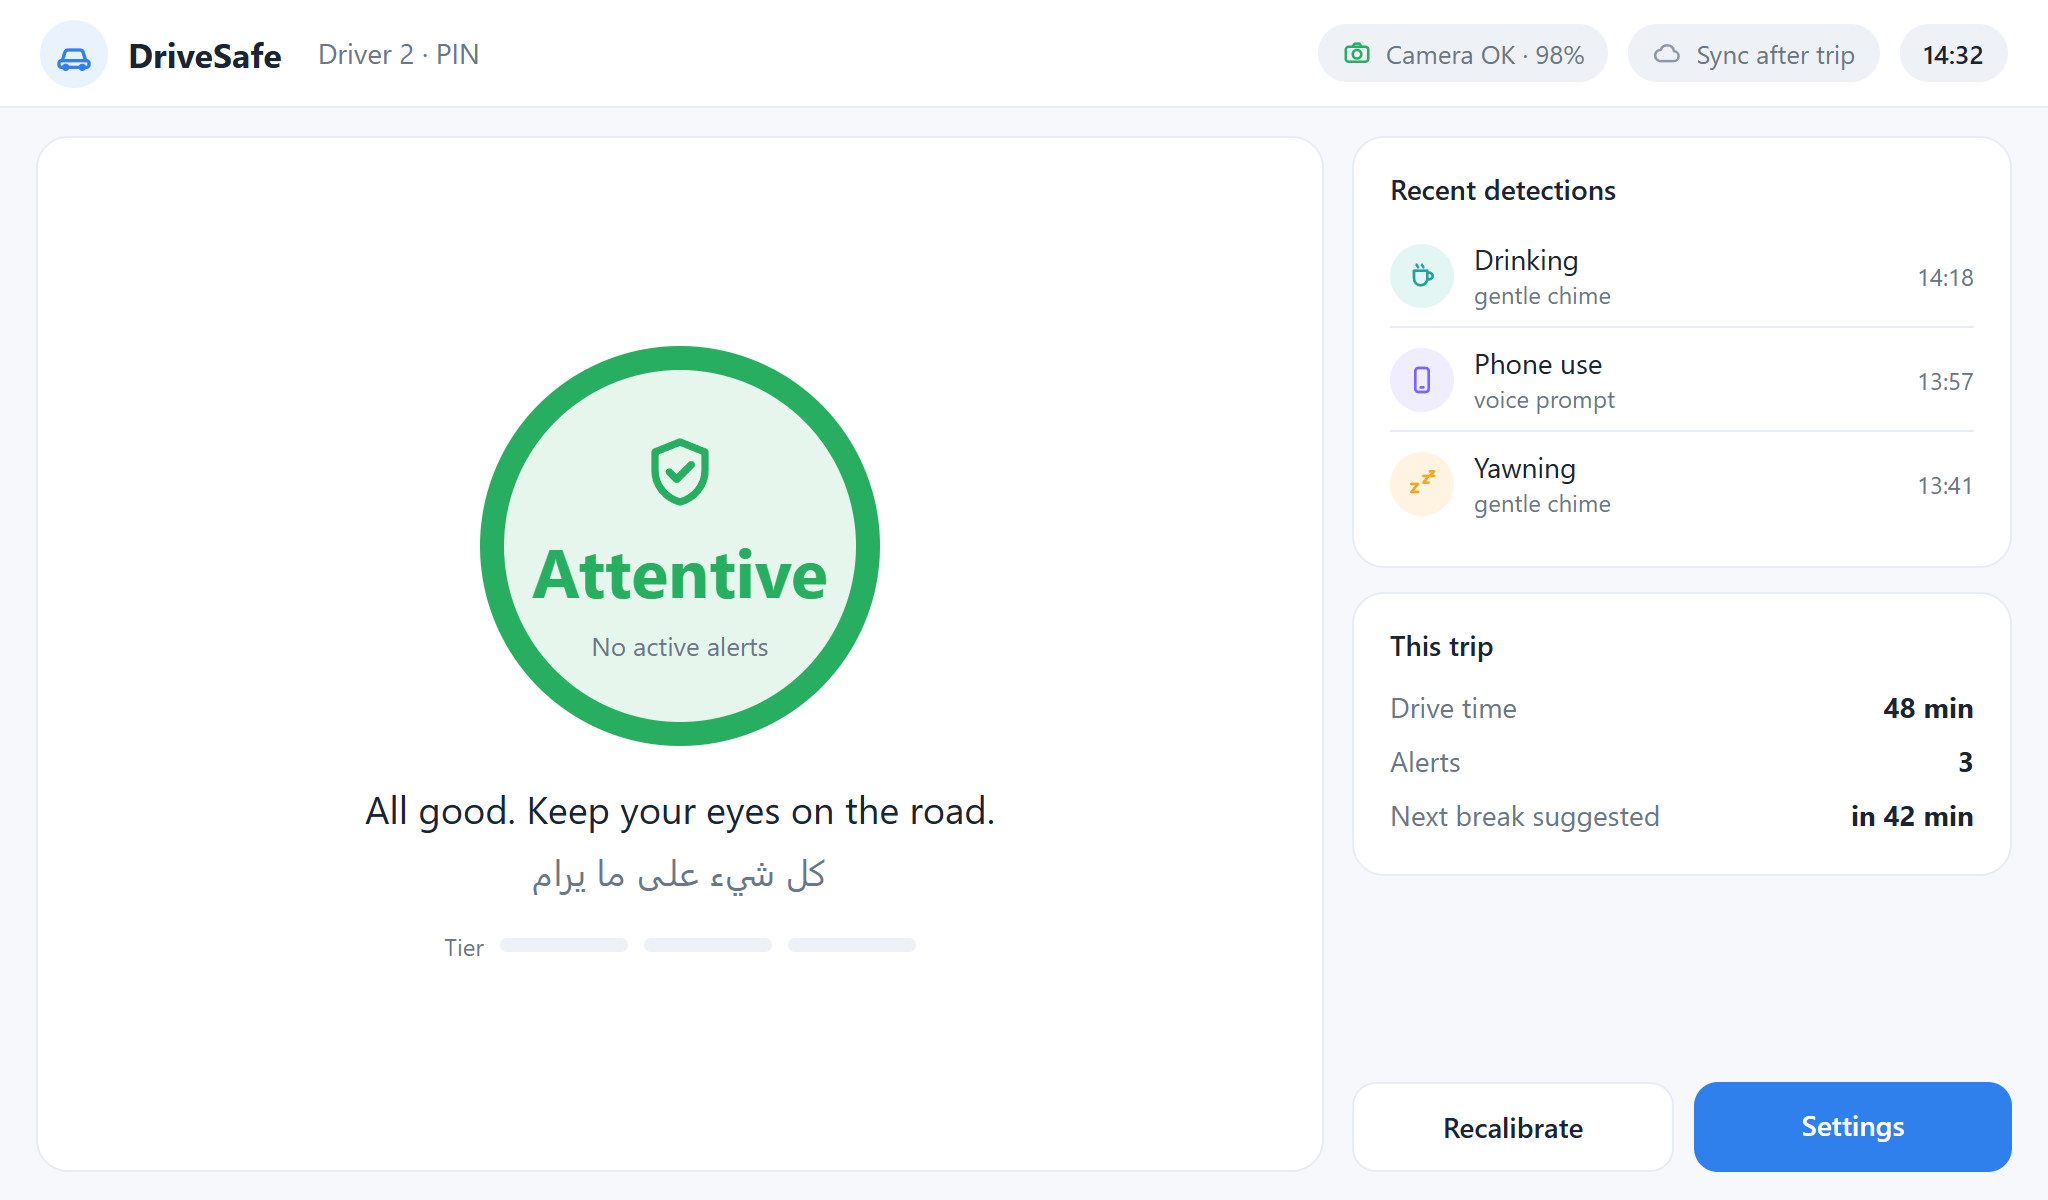
\includegraphics[width=\linewidth]{Figures/ui_tablet_light.png}\caption{Attentive (day)}\end{subfigure}\hfill
\begin{subfigure}[t]{0.49\linewidth}\centering
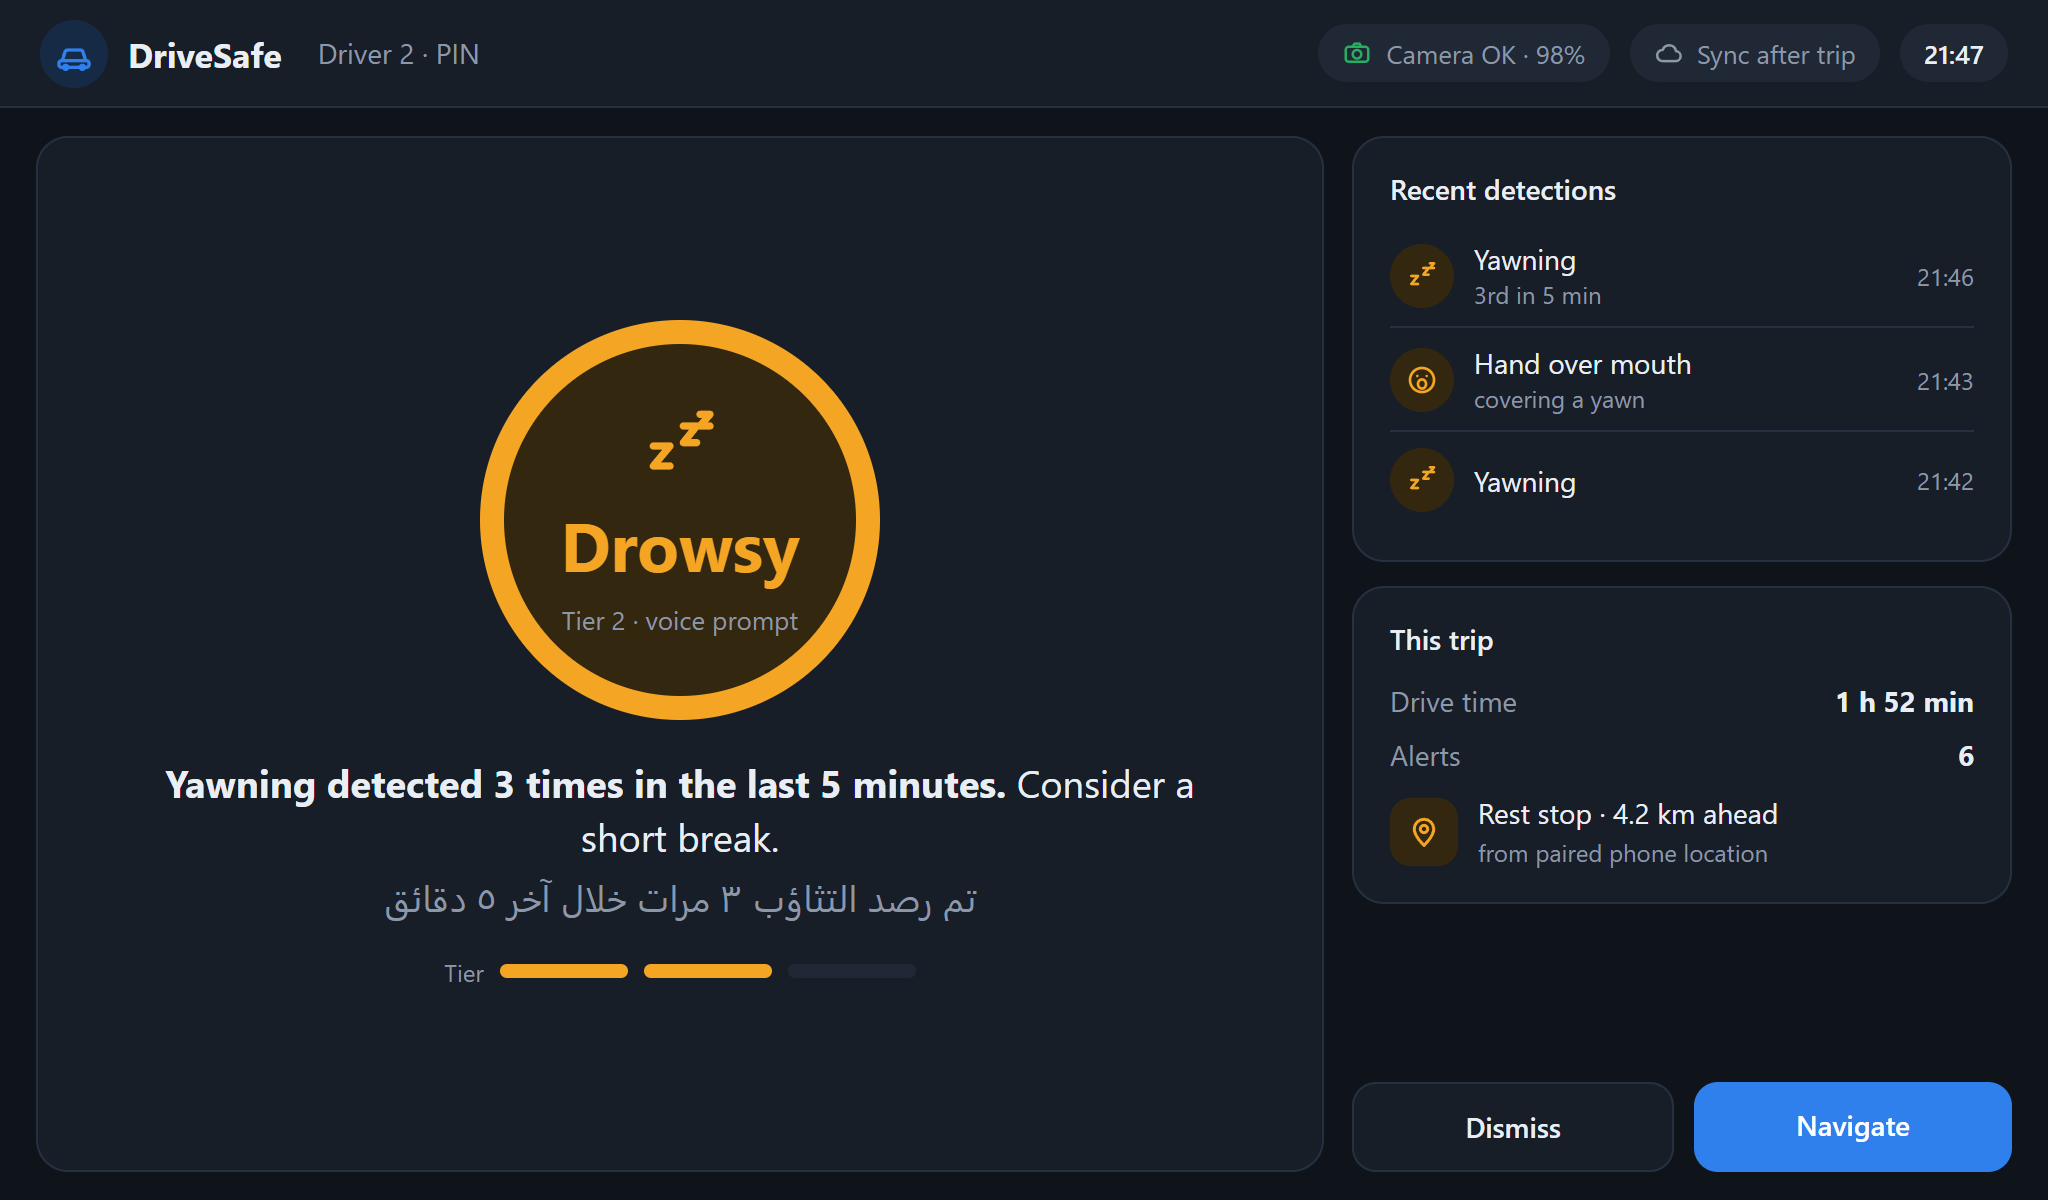
\includegraphics[width=\linewidth]{Figures/ui_tablet_dark.png}\caption{Drowsy, Tier 2 (night)}\end{subfigure}\\[2mm]
\begin{subfigure}[t]{0.49\linewidth}\centering
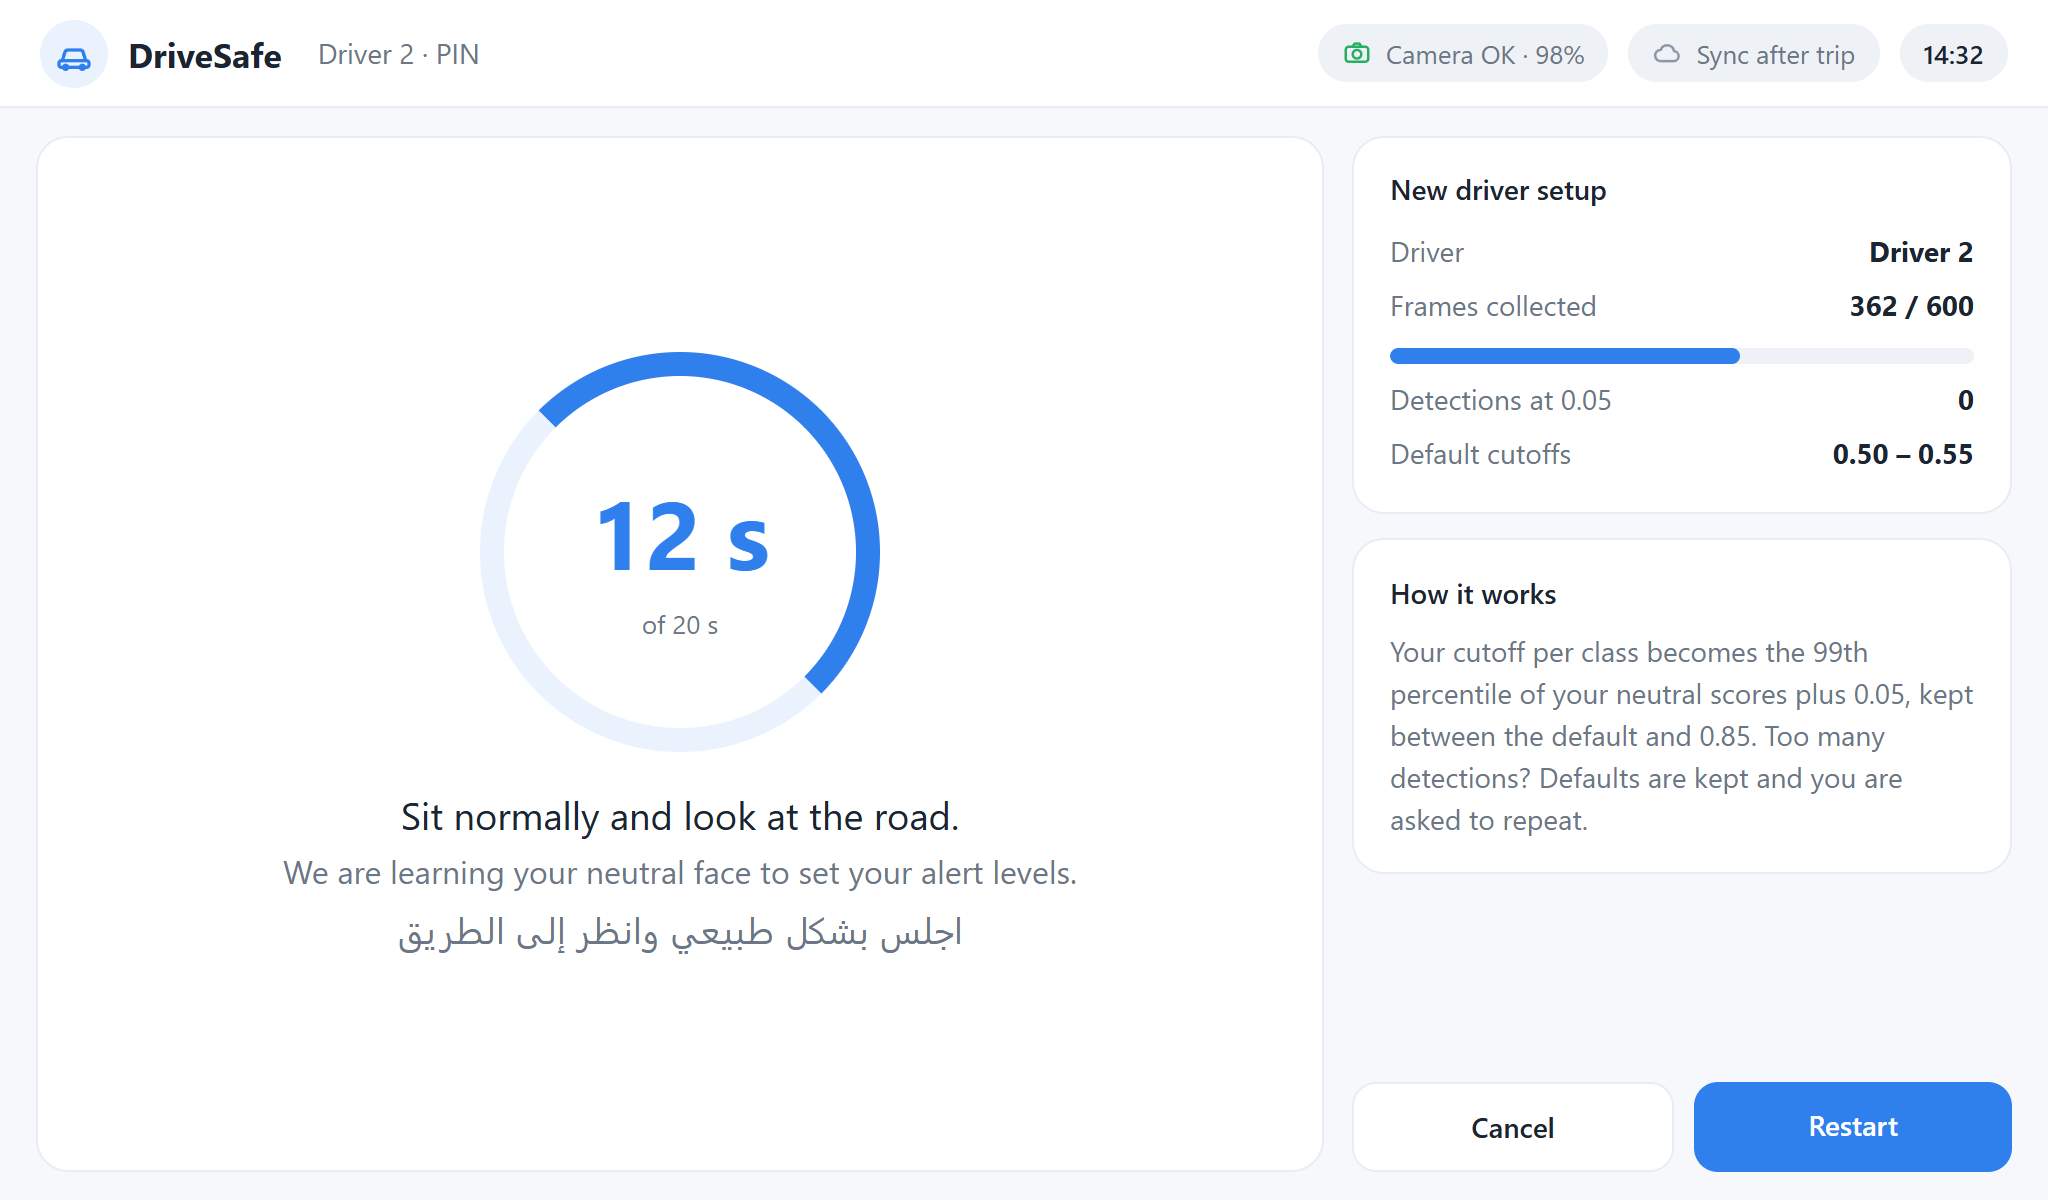
\includegraphics[width=\linewidth]{Figures/ui_tablet_cal.png}\caption{New-driver calibration}\end{subfigure}
\caption{Driver-facing display screens (\glsentryshort{ui} mock-ups)}
\label{fig:ch4-19}
\end{figure}

\subsection{Logging, server and dashboard}
\subsubsection{Power-cut-safe on-device logging}

Events are stored in SQLite with \gls{wal} mode and \texttt{synchronous=NORMAL}, committing each event in a single short transaction, so a power cut cannot corrupt the database, although it may lose the last commits. The schema holds driver, session, event, calibration and tip tables (Figure \ref{fig:ch4-er}), where an event row stores the time, class, confidence, duration, tier and message, along with \texttt{uploaded} and \texttt{escalated} flags. No frames are stored by default. On every boot, \texttt{PRAGMA integrity\_check} runs before a new session starts, and a failed check moves the old file aside and starts a fresh one.

\begin{figure}[htbp]
  \centering
  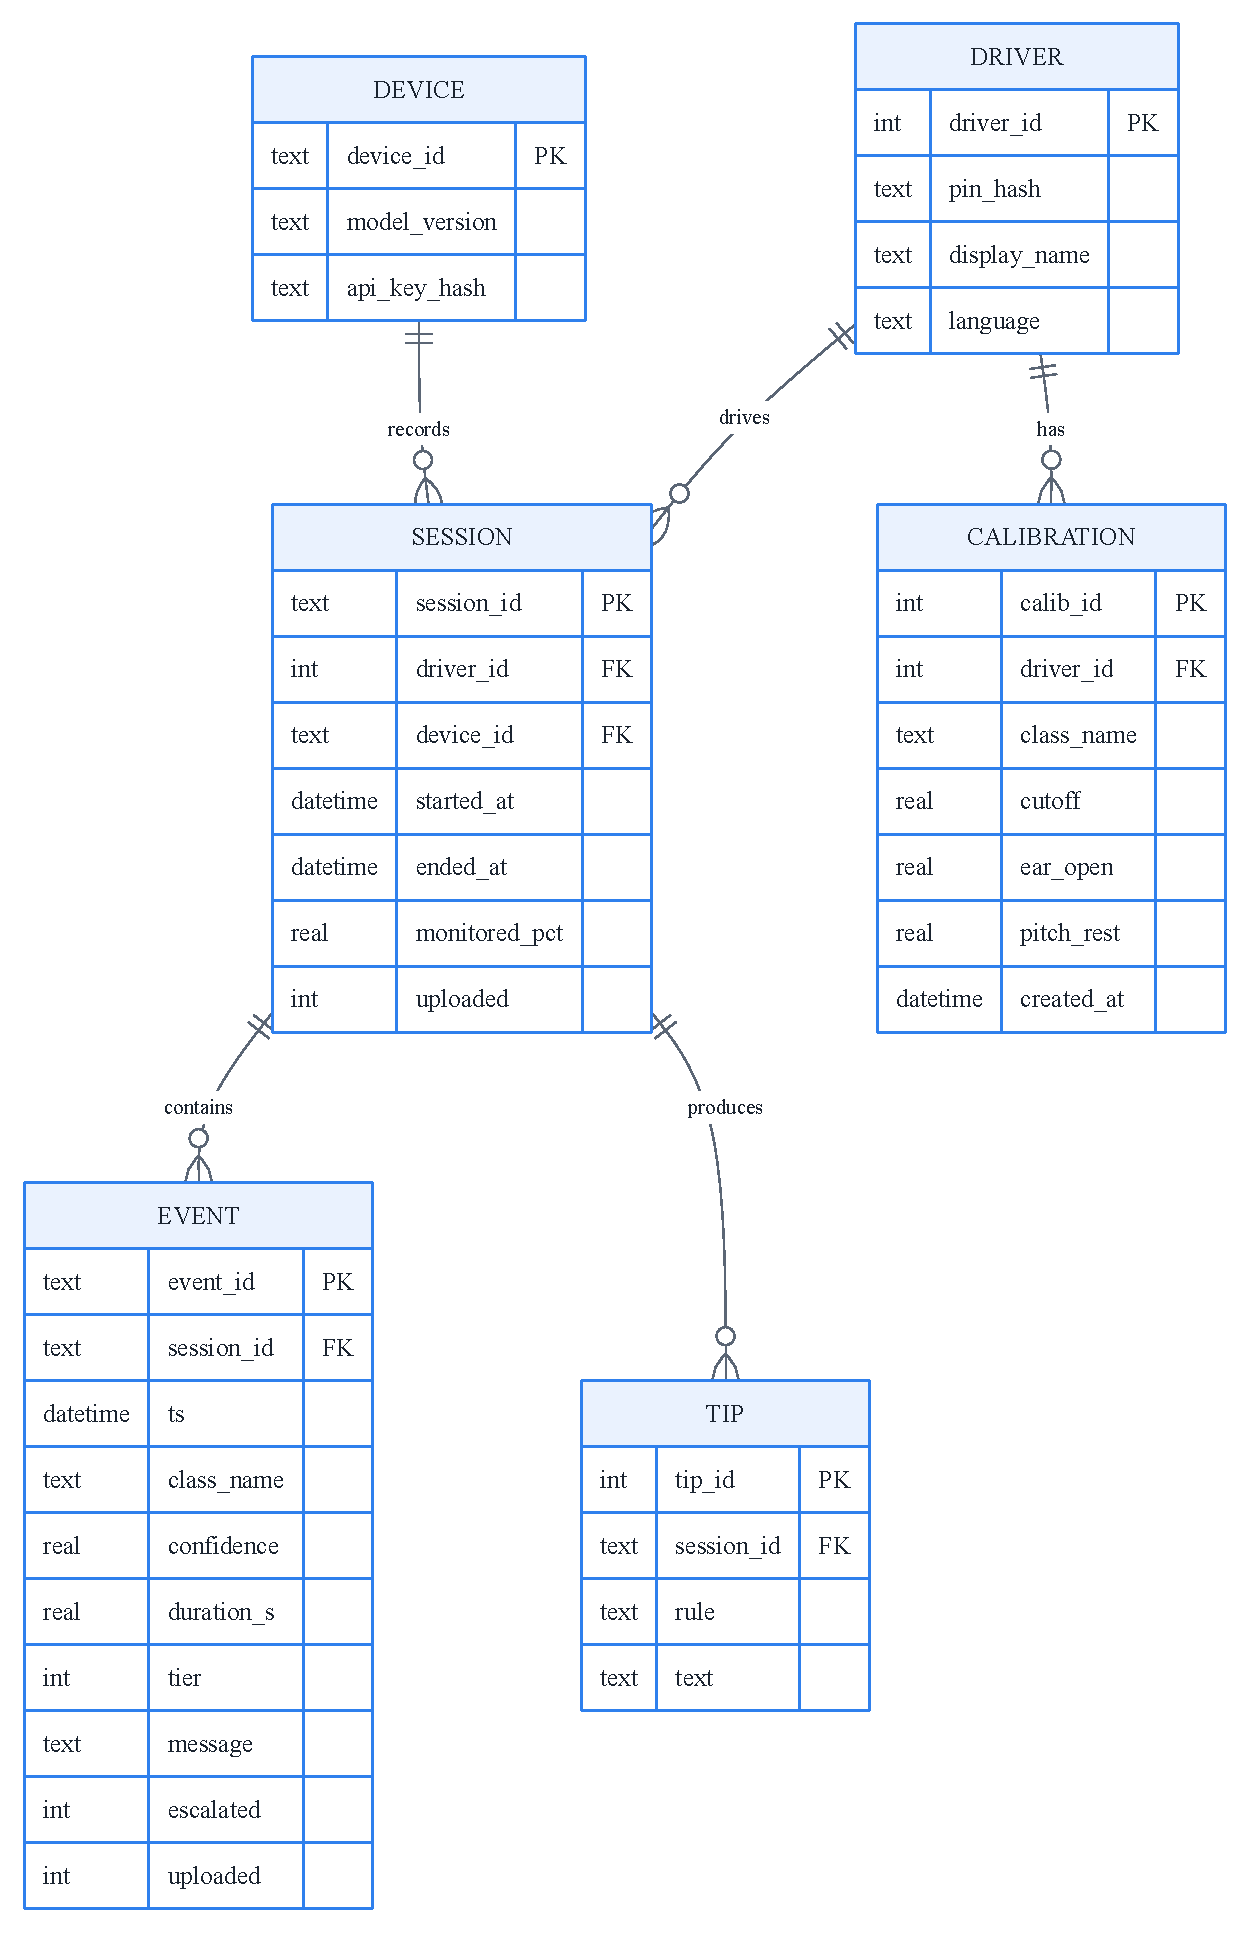
\includegraphics[width=\linewidth, height=0.78\textheight, keepaspectratio]{Figures/uml_er.pdf}
  \caption{Entity-relationship diagram of the event database (same schema on the device and the server)}
  \label{fig:ch4-er}
\end{figure}

\subsubsection{Session upload and server update}

After the session, the uploader selects unsent events and posts them as \gls{json} to the server over HTTPS with \gls{tls} 1.3, authenticated by a per-device key in a request header. Each event carries a random identifier created on the device, allowing the server to ignore duplicates when an upload is retried, and the device marks rows as uploaded only after the server confirms. Failed attempts back off for 30, 60 and 120\,s before waiting for the next session. No frames, embeddings or images are ever sent. Figure \ref{fig:ch4-20} shows the sequence.

\begin{figure}[htbp]
  \centering
  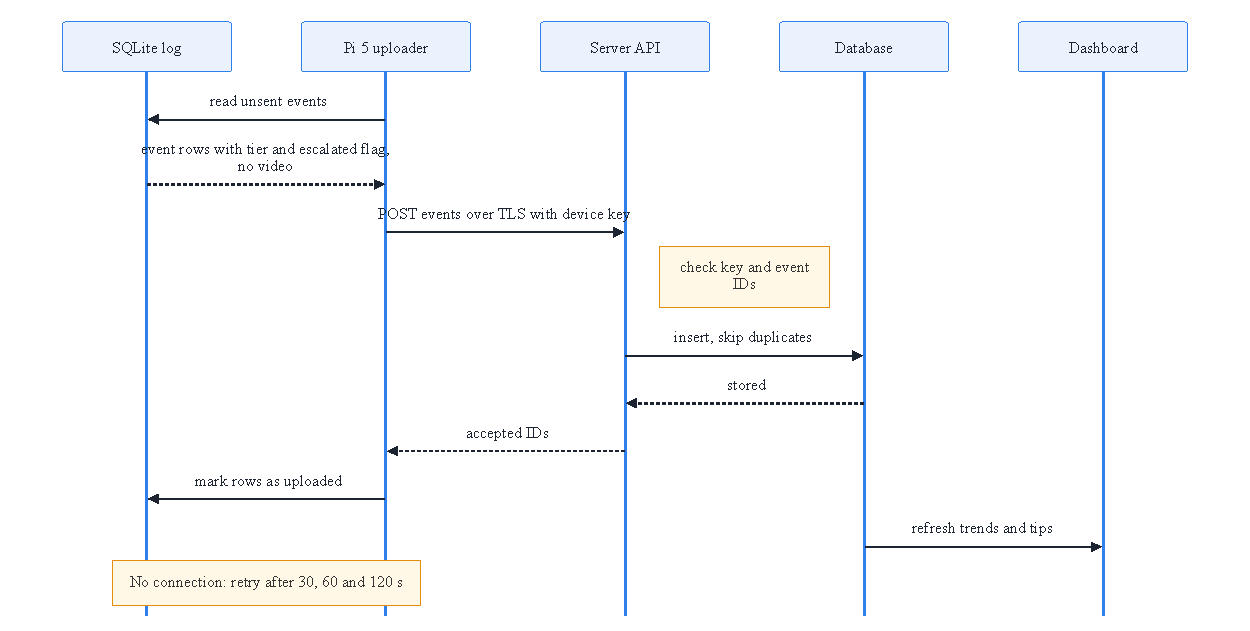
\includegraphics[width=0.9\linewidth]{Figures/uml_seq.pdf}
  \caption{Upload sequence from the Pi to the server and dashboard}
  \label{fig:ch4-20}
\end{figure}

\subsubsection{Web dashboard and post-trip tips}

The dashboard presents the driver's total drive time, distraction and drowsiness counts, the percentage of drive time monitored, a trend line, a breakdown by class, an activity heatmap by weekday and hour, and a timeline of the last trip. Access is limited to the driver's own account, protected by its own password, since \glspl{pin} never leave the device. Post-trip tips are rules over recurring patterns, for example ``yawning rose after 80 minutes on 4 of 7 trips: take a break around 90 minutes'', or ``phone use happened on 5 of your last 7 trips: set navigation before leaving''. Figure \ref{fig:ch4-21} shows the design.

\begin{figure}[htbp]
  \centering
  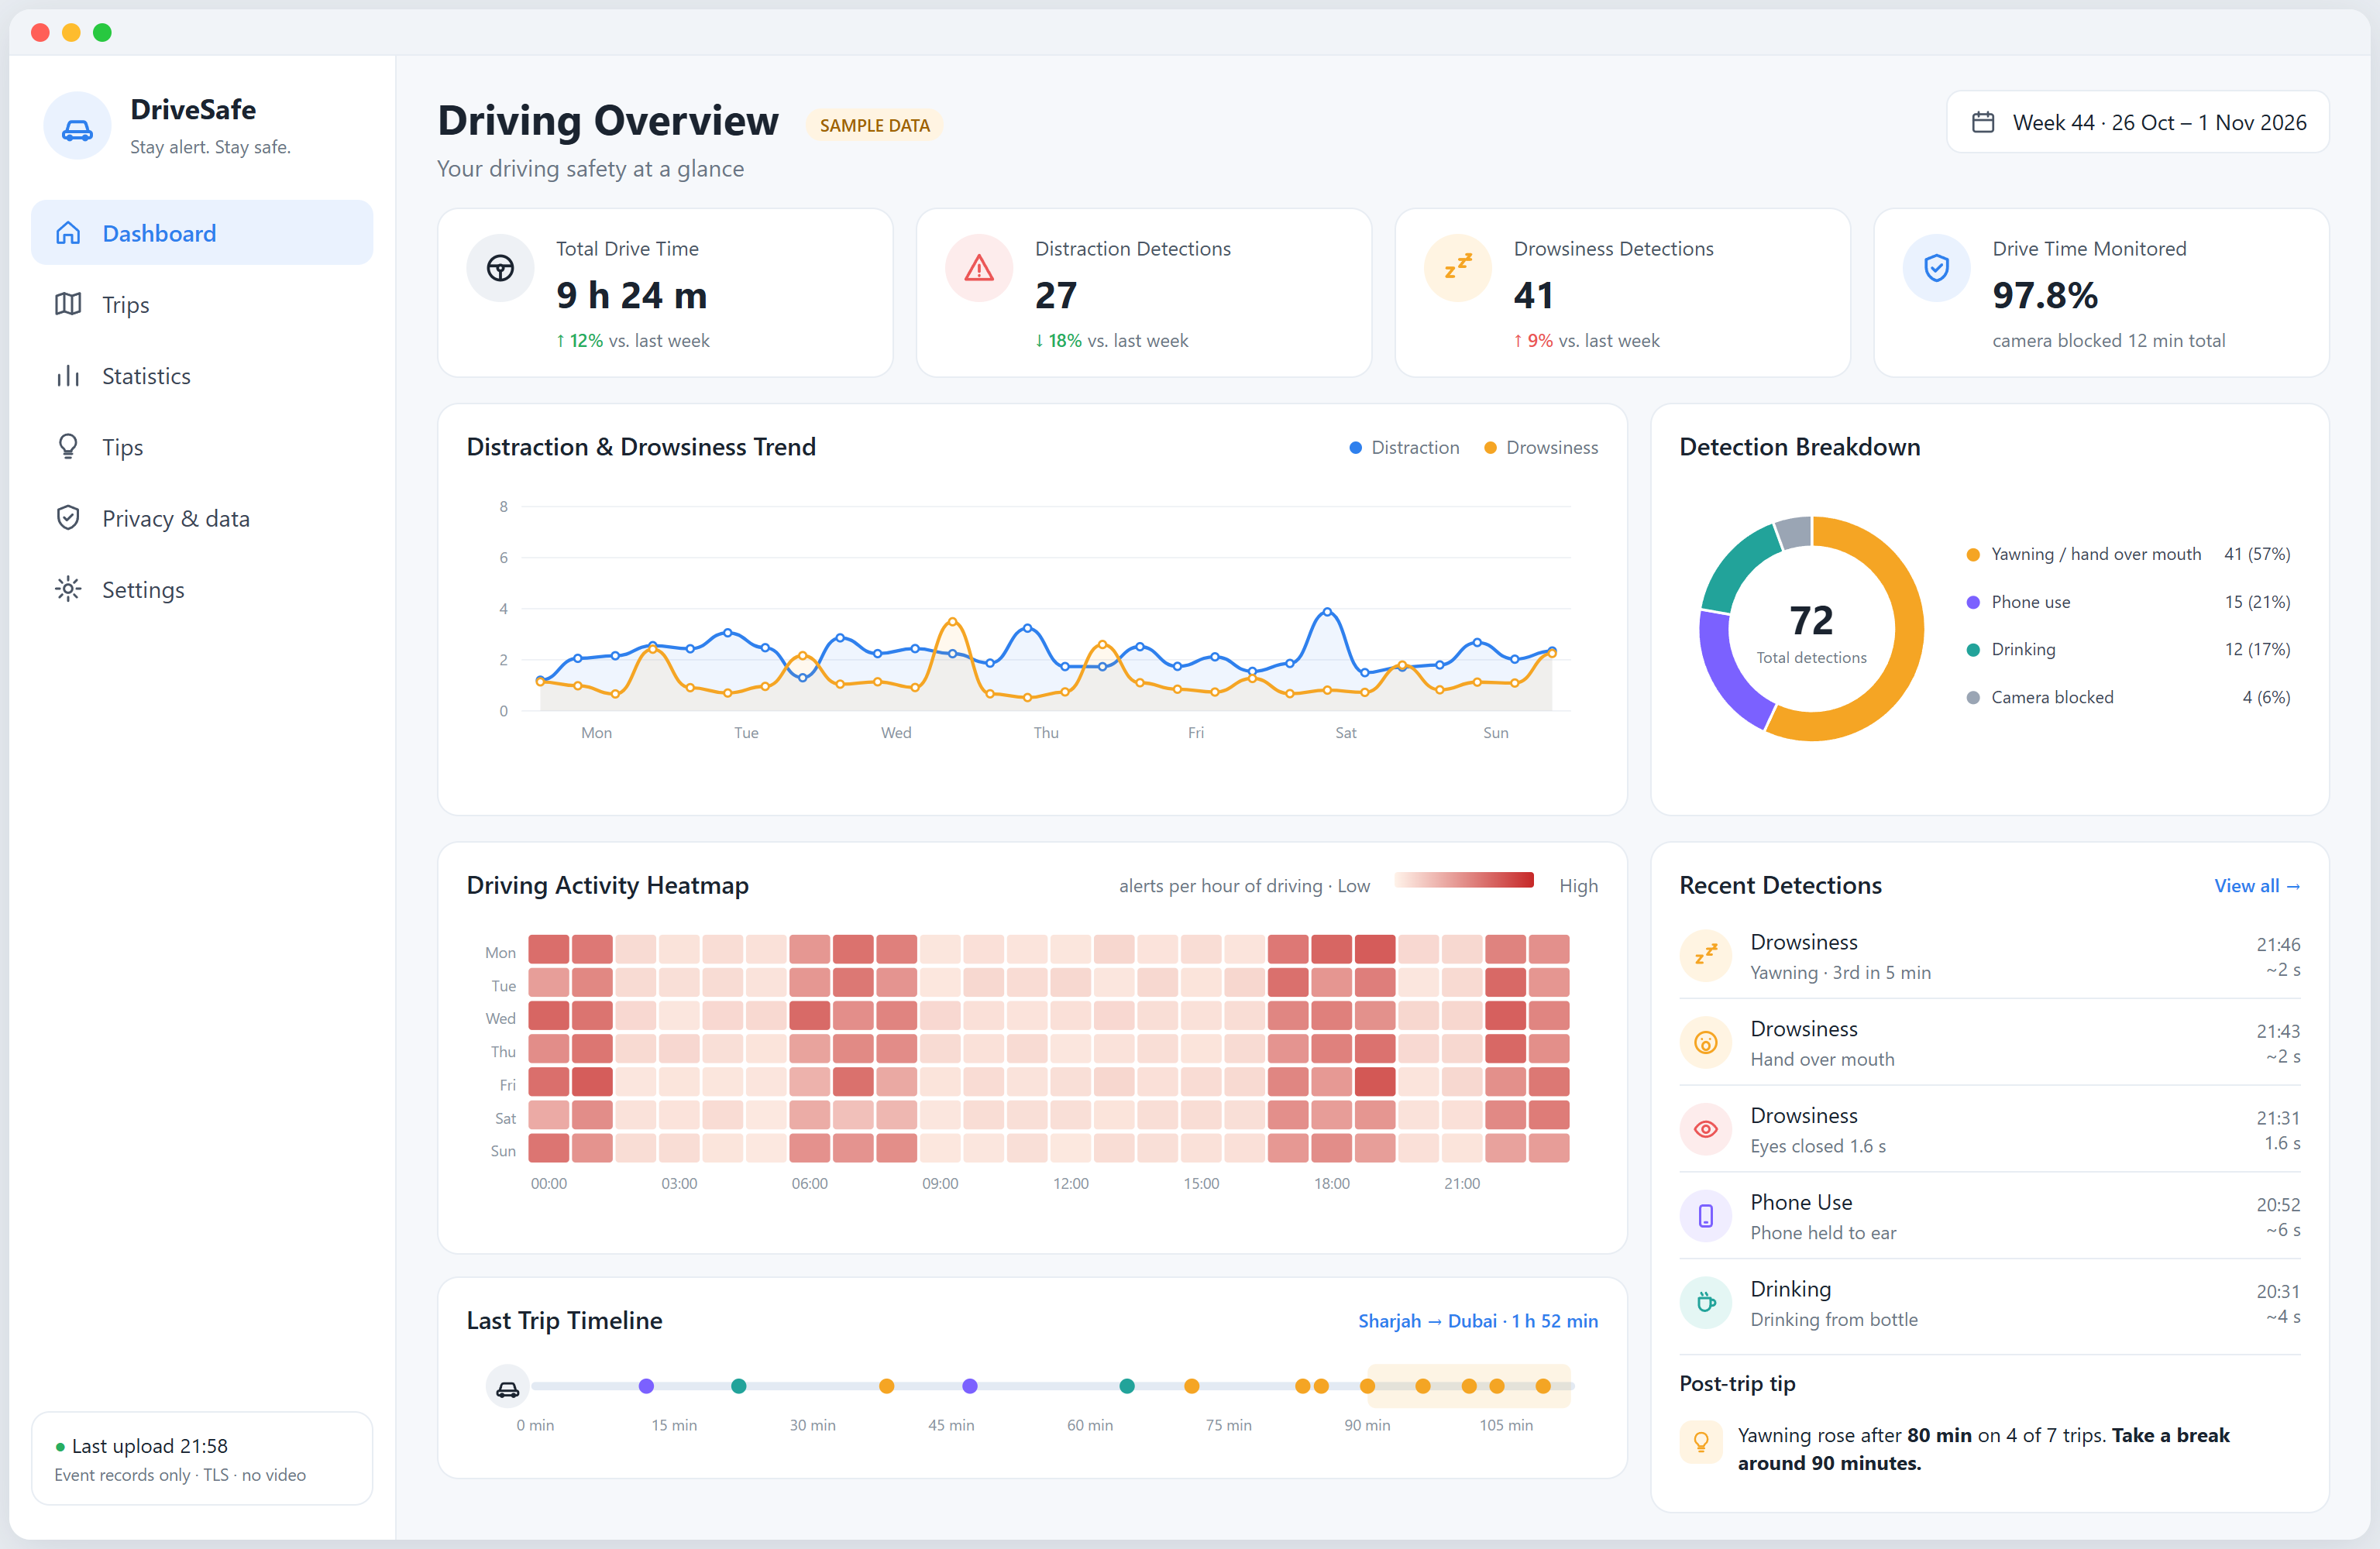
\includegraphics[width=\linewidth]{Figures/ui_dashboard.png}
  \caption{Web dashboard design (sample data)}
  \label{fig:ch4-21}
\end{figure}

\subsection{Calculations, simulations and preliminary results}
\subsubsection{Calculations that justify the design values}

Table \ref{tab:ch4-calc} gives the calculations behind the main design values.

\begin{table}[htbp]
\centering
\caption{Calculations that justify the design values}
\label{tab:ch4-calc}
\footnotesize
\setlength{\tabcolsep}{3pt}
\renewcommand{\arraystretch}{1.15}
\begin{tabular}{|p{0.120\linewidth}|p{0.500\linewidth}|p{0.310\linewidth}|}
\hline
\textbf{Topic} & \textbf{Calculation} & \textbf{Design effect} \\
\hline
\gls{ema} & With $\tau=0.6$\,s, $\alpha=0.054$ at 30 \gls{fps} and 0.105 at 15 \gls{fps}. One spike of $x=1$ gives only 0.054. Reaching 0.5 from zero takes 13 frames, so $t_\theta=-0.6\ln 0.5=0.42$\,s (Equation \ref{eq:delay}) & $\alpha$ must come from $\Delta t$, and single spikes never alert \\
\hline
Compute & 6.5 GFLOPs $\times$ 30 \gls{fps} = 195 GFLOP/s, while the Pi CPU gives about 44 GFLOP/s (6.79 \gls{fps} \cite{r52}). At 320 px the work drops to 1.6 GFLOPs, close to 27 \gls{fps} & The AI HAT+ is Required, with a 320 px CPU fallback \\
\hline
Storage & About 120 bytes per event, so 100 events per day add 4.4 MB per year, and an upload of 100 events is about 20 kB & The 128 GB card and Wi-Fi are far more than enough \\
\hline
Power & 5 V $\times$ 3.25 A = 16.3 W typical on a 25.5 W supply (Table \ref{tab:ch4-13}) & About 9 W of margin \\
\hline
\end{tabular}
\end{table}



Latency is measured from frame capture to the alert command, excluding the deliberate confirmation time. Table \ref{tab:ch4-17} sets a 60 ms target against the 100 ms limit.

\begin{table}[htbp]
\centering
\caption{Latency budget per stage}
\label{tab:ch4-17}
\footnotesize
\hyphenpenalty=10000
\setlength{\tabcolsep}{4pt}
\renewcommand{\arraystretch}{1.15}
\begin{tabular}{|*{6}{>{\raggedright\arraybackslash}p{0.135\linewidth}|}}
\hline
\textbf{Capture, crop} & \textbf{Detection (\glsentryshort{npu})} & \textbf{\glsentryshort{nms}} & \textbf{\glsentryshort{ema} and decision} & \textbf{Alert output} & \textbf{End-to-end} \\
\hline
8 ms & 20 ms & 4 ms & 2 ms & 26 ms & \textbf{60 ms} \\
\hline
\end{tabular}
\end{table}


\subsubsection{Preliminary experiments}

Before the SDP~2 hardware arrives, we conducted four studies on public data using a workstation with an RTX 4060 \gls{gpu}, each released as an open repository \cite{rs1,rs2,rs3,rs4}. Table \ref{tab:prelim} summarises what each study measured and the design decision it informed.

\textbf{Detector choice.} On DMD with a 14-driver subject-disjoint split, \gls{yolo}11n achieved the highest \gls{map}$_{50}$ (0.918) and speed (68 \gls{fps}) of three nano detectors \cite{rs1}. Even so, its F1 ranged from 0.62 to 0.95 between test drivers. The false positive in Figure \ref{fig:ch4-qual}, a tissue held over the mouth, is precisely the kind of look-alike our hard-negative round targets.

\begin{figure}[htbp]
  \centering
  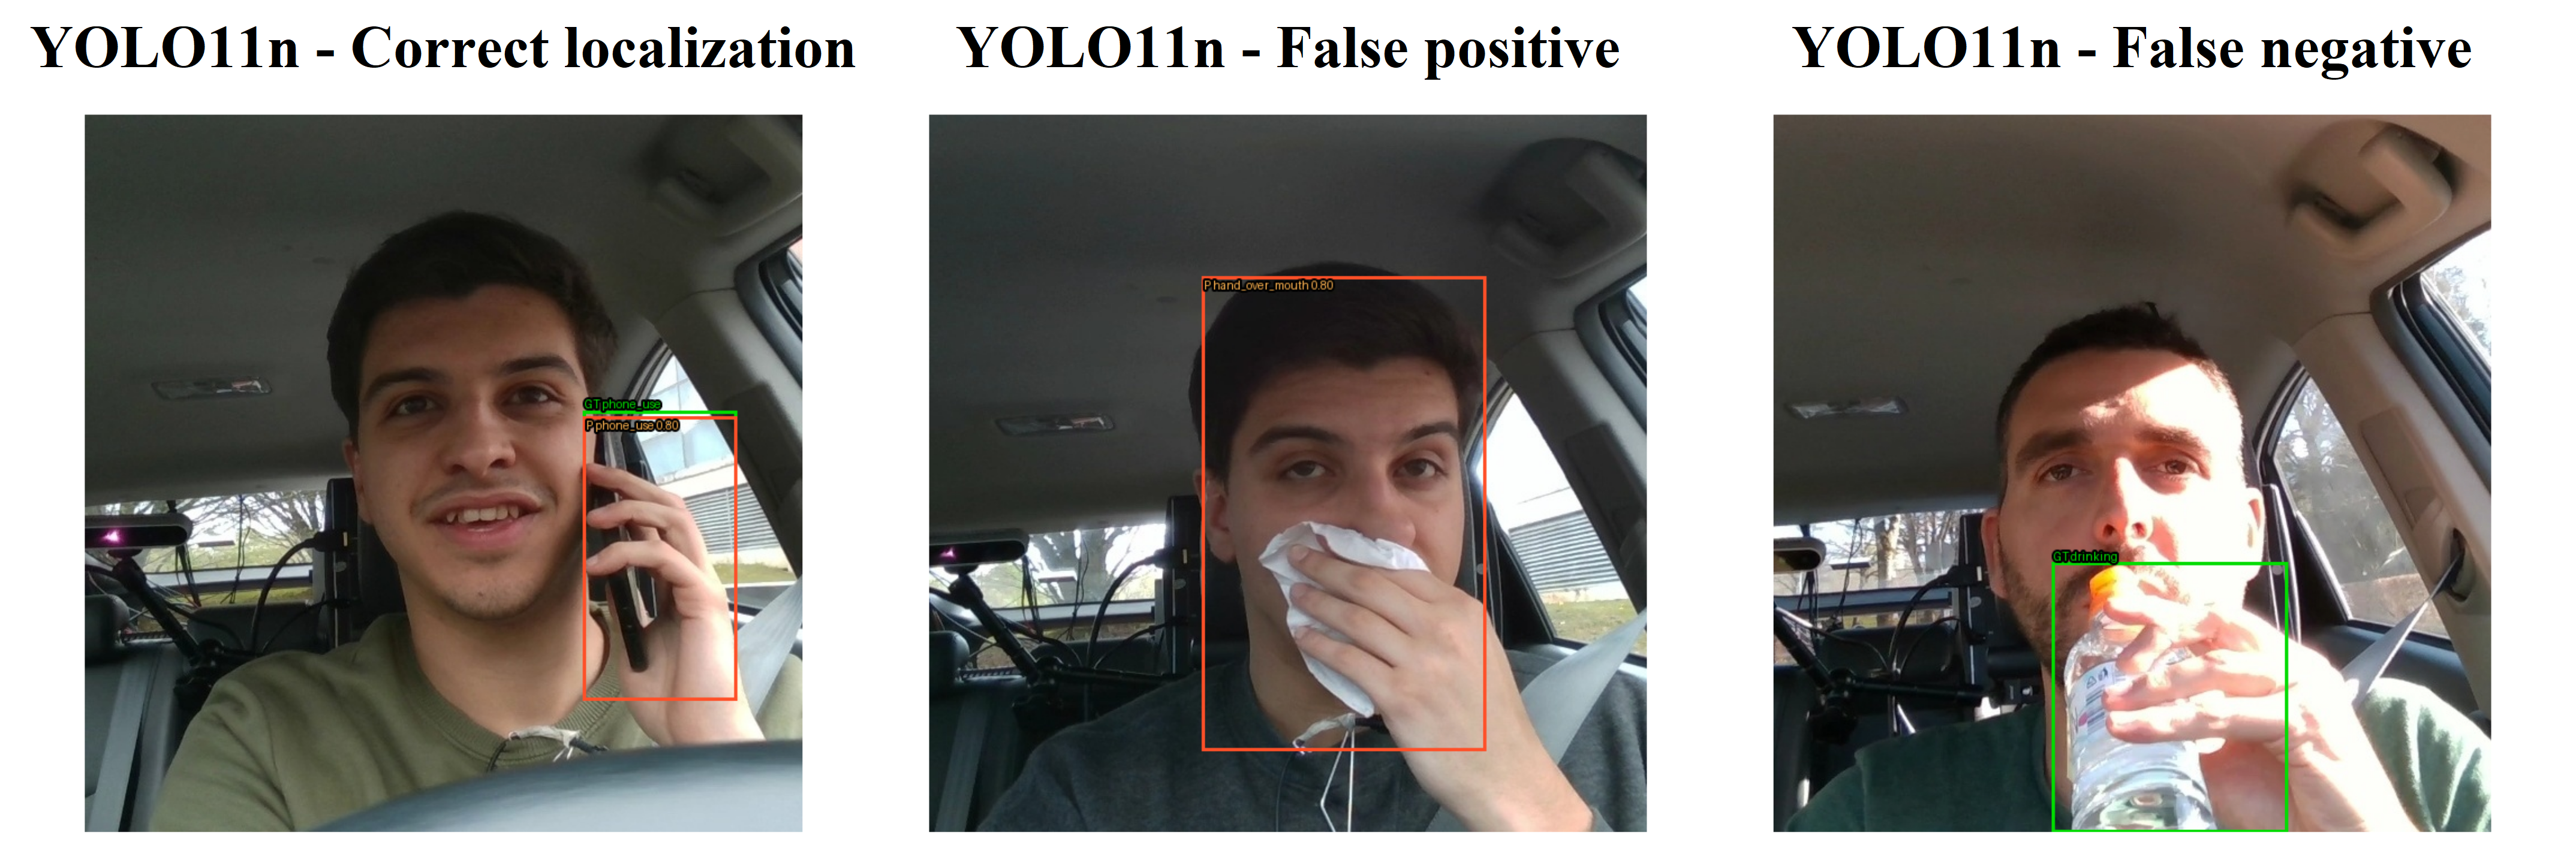
\includegraphics[width=\linewidth]{Figures/rs1_yolo11n_examples.png}
  \caption{\glsentryshort{yolo}11n on held-out DMD drivers: correct detection, false positive and missed detection (from our benchmark \cite{rs1})}
  \label{fig:ch4-qual}
\end{figure}

Figure \ref{fig:ch4-weak} highlights two weak cells. Hand-over-mouth precision is only 0.54 due to look-alikes, and one held-out driver is detected only half of the time, which is why we mine hard negatives and always evaluate on unseen drivers.

\begin{figure}[htbp]
  \centering
  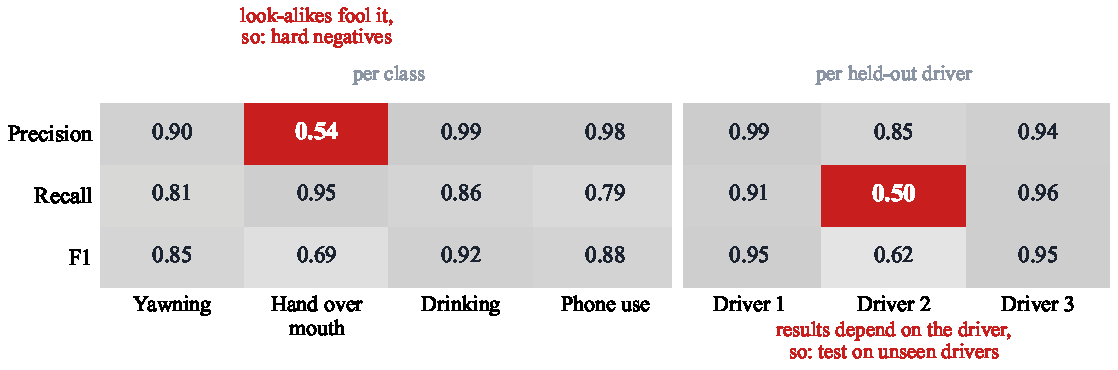
\includegraphics[width=\linewidth]{Figures/heat_yolo_weak.pdf}
  \caption{Where \glsentryshort{yolo}11n is weak: precision, recall and F1 per class and per held-out DMD driver, mean of three seeds \cite{rs1}}
  \label{fig:ch4-weak}
\end{figure}

\textbf{False alarms and cropping.} Both studies are presented in Chapter 1 (Figure \ref{fig:empirical_studies}): 40\% hard-mined negatives cut false positives by 71\% \cite{rs2}, and cropping to the driver preserves accuracy down to 320 px.

\textbf{Compression and cutoffs.} Structured pruning of up to 50\% kept the per-class AP$_{50}$ of \gls{yolo}11n within about two points (\gls{map}$_{50}$ from 0.933 to 0.928), yet at a fixed cutoff of 0.5 its worst-class recall fell by 6.8 points. Cutoffs tuned on validation drivers met a recall floor on unseen test drivers in at most one of three training seeds, and \gls{int} quantization with TensorRT lowered \gls{map}$_{50}$ from 0.933 to 0.874 \cite{rs3}.

\textbf{Temporal filtering.} In our RGB-thermal detection study, a five-frame moving average reduced false alerts from 9.0 to 2.1 per minute compared with raw thresholding, at the cost of about 0.4\,s of extra delay, while learned temporal models (GRU and Mamba) were not significantly better and ran up to 500 times slower \cite{rs4}.


\begin{table}[htbp]
\centering
\caption{Preliminary studies and the design decision each one supports}
\label{tab:prelim}
\footnotesize
\setlength{\tabcolsep}{3pt}
\renewcommand{\arraystretch}{1.15}
\begin{tabular}{|p{0.170\linewidth}|p{0.190\linewidth}|p{0.320\linewidth}|p{0.250\linewidth}|}
\hline
\textbf{Study} & \textbf{Data} & \textbf{Main result} & \textbf{Design decision} \\
\hline
Detector benchmark \cite{rs1} & DMD, 14 drivers, subject-disjoint & \gls{yolo}11n best \gls{map}$_{50}$ (0.918) and speed of three nano detectors & \gls{yolo}11n selected \\
\hline
Negatives and hard negatives \cite{rs2} & 15{,}723 frames & 40\% hard-mined negatives: 24.4 $\rightarrow$ 7.1 false positives per 1000 frames & Hard-negative round (FS-12) \\
\hline
Pruning and quantization \cite{rs3} & DMD, our four classes & AP kept up to 50\% pruning, cutoffs fail across drivers and \gls{int} costs 5.9 \gls{map}$_{50}$ points & Per-driver calibration (FS-19), comparing \gls{ptq} and \gls{qat} \\
\hline
Temporal filtering \cite{rs4} & RGB-thermal video & Moving average: 9.0 $\rightarrow$ 2.1 false alerts per minute & Simple time-based \gls{ema} (FS-04) \\
\hline
\gls{roi} cropping (Chapter 1) & Public DMS data & Crop keeps accuracy down to 320 px, $\le$ 3 ms & Fixed crop, 320 px CPU fallback \\
\hline
\end{tabular}
\end{table}

\subsubsection{What the results tell us}

Together, the studies support \gls{yolo}11n, hard-negative mining and a simple time-based average. Most importantly, a cutoff tuned on some drivers does not hold for others, forming the strongest argument for per-driver calibration. The main risks are the \gls{int} accuracy drop on the \gls{npu} and how well results on public data transfer to our own recordings of the four authors.

\section{Real-World Considerations}

\subsection{Environmental impact}

The device adds a small amount of e-waste in the Pi, the HAT, the camera, the hub and the display, but contains no battery to dispose of, and at about 16 W it consumes less energy than a car's headlights. Training is the largest energy cost, which we limit by fine-tuning a small pre-trained model rather than training from scratch, and by running compression only once. The server stores only small event records, keeping its energy use minimal. At the end of the project, the parts are returned to the university lab for reuse.

\subsection{Ethical and social issues in the UAE context}
\label{sec:ethics}
\subsubsection{Privacy}

Our own dataset records only the four authors (Section \ref{sec:dataset}), so no outside participants are involved. For a product, every driver would give consent under the \gls{uae} \gls{pdpl} \cite{r56}, with \gls{gdpr} \cite{r57} as a reference, and a ``delete my data'' button on the dashboard remains a Future item.

\subsubsection{Social and cultural perception in the UAE}

An in-car camera can feel intrusive, especially for families and for women who may prefer not to be filmed. Keeping all video on the device and never uploading it is our main answer, together with a visible camera that is never hidden. Fleet employees, such as taxi drivers, may fear the system being used to punish them, so our design gives the data to the driver first and shares only events, never video. Voice messages in both Arabic and English make the system feel local and clear, and since phone use costs 800 \gls{aed} and four black points in the \gls{uae} \cite{r65}, drivers have a personal reason to welcome a gentle reminder.

\subsubsection{Fairness and responsible use}

Detection quality may differ for drivers with glasses, headscarves, beards or different skin tones. With only the four authors in our own dataset, we cannot measure this ourselves, so we fine-tune on the 14 drivers of DMD first and report results per driver, leaving a larger and more varied test set as a Future item. Alert fatigue is itself a safety risk, which is precisely why the cool-down, calibration and tiered alerts exist. The system is designed to assist and explain rather than punish, giving tips instead of scores, and it is never presented as a replacement for the driver's attention.

\subsection{Economic analysis}
\subsubsection{Cost to produce}

The prototype costs 2725 \gls{aed}, of which the 250 \gls{aed} wheel serves the demonstration rig and the haptic prototype. A single unit costs about 2160 \gls{aed} without the display, and a custom board with the same \gls{npu} could bring this below 800 \gls{aed} at volume. Cloud costs stay small, as only events are uploaded (Table \ref{tab:ch4-19}).

\begin{table}[htbp]
\centering
\caption{Unit cost and cloud cost}
\label{tab:ch4-19}
\footnotesize
\setlength{\tabcolsep}{3pt}
\renewcommand{\arraystretch}{1.15}
\begin{tabular}{|p{0.316\linewidth}|p{0.307\linewidth}|p{0.307\linewidth}|}
\hline
\textbf{Quantity} & \textbf{BOM per unit (\gls{aed})} & \textbf{Cloud cost / month} \\
\hline
1 unit, without display & About 2160 & Free tier \\
\hline
1 unit, with display & About 2475 & Free tier \\
\hline
Volume (1000+ units, custom board) & Below 800 (estimate) & About 1--2 \gls{aed} per driver \\
\hline
\end{tabular}
\end{table}

\subsubsection{What makes our product competitive}

Unlike the products of Section 2.3, our device is a one-off purchase that works in any car, gives the feedback to the driver, keeps video on the device, reports false alarms per hour and calibrates per driver. In a production vehicle, each prototype part has an existing equivalent: an \gls{nir} camera in the cluster, a driver-assistance computer with an \gls{npu}, an ambient \gls{led} strip, the cabin speakers and a haptic steering wheel. Table \ref{tab:ch4-20} summarises the strengths and risks.

\begin{table}[htbp]
\centering
\caption{SWOT analysis}
\label{tab:ch4-20}
\footnotesize
\setlength{\tabcolsep}{4pt}
\renewcommand{\arraystretch}{1.2}
\begin{tabular}{|p{0.45\linewidth}|p{0.45\linewidth}|}
\hline
\cellcolor{out1!15}\textbf{Strengths} & \cellcolor{oth1!15}\textbf{Weaknesses} \\
\hline
Low cost with no subscription, video never leaves the car, explained and tiered alerts, per-driver calibration and open evaluation & \gls{rgb} only and weak at night, four classes only, and a bench prototype not certified for vehicles \\
\hline
\cellcolor{own1!15}\textbf{Opportunities} & \cellcolor{oth2!20}\textbf{Threats} \\
\hline
\gls{eu} \gls{gsr} mandates raise awareness, \gls{uae} fleets (taxis, \gls{rta}), a retrofit market for older cars and an Arabic-first interface & Factory-fitted systems in new cars, the AGPL licence if commercialised and driver acceptance of in-car cameras \\
\hline
\end{tabular}
\end{table}
